% ============================================================
% Agent Control Protocol — arXiv Submission
% ACP v1.20 — Admission Control for Agent Actions
% Marcelo Fernandez, TraslaIA, March 2026
% Categories: cs.CR (primary), cs.AI (secondary)
% ============================================================

\documentclass[11pt]{article}

% --- Encoding & fonts ---
\usepackage[utf8]{inputenc}
\usepackage[T1]{fontenc}
\usepackage{lmodern}
\usepackage{microtype}

% --- Page geometry ---
\usepackage[margin=1in, top=1.1in, bottom=1.1in]{geometry}

% --- Math ---
\usepackage{amsmath,amssymb}

% --- Tables ---
\usepackage{booktabs}
\usepackage{tabularx}
\usepackage{longtable}
\usepackage{array}
\usepackage{multirow}

% --- Code listings ---
\usepackage{listings}
\usepackage{xcolor}

\definecolor{codegray}{rgb}{0.5,0.5,0.5}
\definecolor{codegreen}{rgb}{0,0.5,0}
\definecolor{codeblue}{rgb}{0,0,0.6}
\definecolor{codebg}{rgb}{0.97,0.97,0.97}

\lstdefinestyle{acp}{
  backgroundcolor=\color{codebg},
  basicstyle=\small\ttfamily,
  breakatwhitespace=false,
  breaklines=true,
  captionpos=b,
  commentstyle=\color{codegray}\itshape,
  frame=single,
  framesep=4pt,
  keepspaces=true,
  keywordstyle=\color{codeblue}\bfseries,
  numbers=none,
  numberstyle=\tiny\color{codegray},
  showspaces=false,
  showstringspaces=false,
  showtabs=false,
  stringstyle=\color{codegreen},
  tabsize=2,
  columns=flexible
}

\lstset{style=acp}

% --- Hyperlinks ---
\usepackage{hyperref}
\hypersetup{
  colorlinks=true,
  linkcolor=blue!70!black,
  urlcolor=blue!70!black,
  citecolor=blue!70!black,
  pdftitle={Agent Control Protocol: Admission Control for Agent Actions},
  pdfauthor={Marcelo Fernandez},
  pdfsubject={Formal protocol for governance of autonomous agents. v1.20. arXiv:2603.18829},
  pdfkeywords={autonomous agents, admission control, capability tokens, cryptographic governance, agent authorization, audit ledger}
}

% --- Section formatting ---
\usepackage{titlesec}
\titleformat{\section}{\large\bfseries}{\thesection}{1em}{}
\titleformat{\subsection}{\normalsize\bfseries}{\thesubsection}{1em}{}

% --- Spacing ---
\usepackage{setspace}
\setlength{\parskip}{0.5em}
\setlength{\parindent}{0pt}

% --- Diagrams ---
\usepackage{tikz}
\usetikzlibrary{arrows.meta,positioning}
\usepackage{pgfplots}
\pgfplotsset{compat=1.18}

% --- Misc ---
\usepackage{graphicx}
\usepackage{enumitem}
\usepackage{footnote}

% --- Comparison table symbols ---
\newcommand{\yes}{\checkmark}
\newcommand{\no}{$\times$}

% ============================================================
\begin{document}
% ============================================================

\title{%
  \textbf{Agent Control Protocol}\\[0.4em]
  \large ACP v1.20: Admission Control for Agent Actions\\[0.3em]
  \normalsize Technical Specification and Reference Implementation%
}

\author{
  Marcelo Fernandez\\
  TraslaIA\\
  \texttt{info@traslaia.com}\\
  \url{https://agentcontrolprotocol.xyz}
}

\date{March 2026 \\ \small Draft Standard \\ \small \href{https://arxiv.org/abs/2603.18829}{arXiv:2603.18829 [cs.CR]} \quad \href{https://doi.org/10.5281/zenodo.19219776}{DOI: 10.5281/zenodo.19219776}}

\maketitle

% ============================================================
\begin{abstract}
% ============================================================
ACP defines a deterministic admission control protocol for autonomous agents, combining
capability, resource, and temporal signals (history, anomaly, cooldown) into runtime admission
decisions that existing stateless frameworks (RBAC, ABAC, OPA, Cedar) cannot enforce.
The key design insight is that the protocol is \textbf{compute-cheap but state-sensitive}:
decision evaluation is computationally inexpensive ($\sim$820~ns), while system performance
is primarily constrained by state access patterns---a separation that allows the state backend
to be replaced or scaled without modifying protocol semantics.
Experimental evaluation demonstrates throughput up to $\sim$920k~req/s under moderate
concurrency, with the cooldown containment path at $\sim$88~ns (9.5$\times$ faster via
Step~2 early exit), and throughput degrading gracefully to $\sim$712k~req/s at 500 workers
due to state backend contention.
Adversarial evaluation across four attack scenarios---cooldown evasion,
distributed multi-agent coordination, state backend stress, and token replay---confirms
that ACP-RISK-2.0 enforcement holds under active evasion: 99\% (495/500) of
single-agent evasion attempts are blocked after only five requests (Experiment~1),
per-agent isolation is preserved across 100 coordinated agents, throughput
degradation under stress is attributable solely to state-backend latency rather than decision logic,
and repeated identical tokens trigger F\_anom Rule~3 escalation from ESCALATED to DENIED
after three occurrences in a 5-minute window (Experiment~4).
ACP provides end-to-end verifiability through 73~signed conformance test vectors,
a TLC-checked TLA+~formal model (3~invariants, 0~violations), and an ACR-1.0 sequence
compliance runner that validates stateful multi-step behavior at runtime.

\textbf{Specification and implementation:} \url{https://github.com/chelof100/acp-framework-en}
\end{abstract}

\tableofcontents

\newpage

% ============================================================
\section{The Problem ACP Solves}
% ============================================================

Autonomous agents are being deployed in institutional environments without a technical standard to govern their behavior.
This is not a tooling problem---it is a protocol problem.

\subsection{The Structural Gap}

When an autonomous agent makes a decision and executes it, there is a critical moment between both actions.
In current models, that moment does not formally exist: the decision and the execution are the same event.
The agent decides and acts. There is no intermediate validation.
There is no point of intervention. There is no structured record of why the decision was made.

This is acceptable when a human executes that action, because the human bears responsibility and can be questioned.
An autonomous agent cannot be questioned. It can only be audited---and only if there is something to audit.

\begin{quote}
\textit{The problem is not whether agents are trustworthy.
The problem is that currently no formal technical mechanism exists that allows an institution to demonstrate that its agents operated within authorized limits.}
\end{quote}

\subsection{ACP as Admission Control}

The clearest frame for understanding what ACP does is the Kubernetes Admission Controller analogy.

Kubernetes intercepts every API request before it reaches the cluster and runs it through a sequence of admission checks---\texttt{ValidatingWebhookConfiguration},
\texttt{ResourceQuota} enforcement, OPA Gatekeeper policies.
If any check fails, the request is rejected before touching cluster state.

ACP applies this pattern to agent actions:

\begin{lstlisting}
agent intent
    |
[1] Identity check     (ACP-AGENT-1.0, ACP-HP-1.0)
    |    is this agent who they claim to be?
[2] Capability check   (ACP-CT-1.0, ACP-DCMA-1.1)
    |    does the agent hold a valid token for this action?
[3] Policy check       (ACP-RISK-2.0, ACP-PSN-1.0)
    |    is this action within current policy?
[4] ADMIT / DENY / ESCALATE
    |    (if ADMIT)
[5] Execution token    (ACP-EXEC-1.0)
    |    single-use cryptographic proof of admission
[6] Ledger record      (ACP-LEDGER-1.3)
    |    immutable signed audit entry
system state mutation
\end{lstlisting}

The critical difference from Kubernetes: ACP's admission check operates across institutional boundaries.
An agent from Bank~A can be admitted by Bank~B without Bank~B trusting Bank~A's internal infrastructure---the
cryptographic proof is self-contained and verifiable with Bank~A's published public key alone.

This \emph{admission control} framing also clarifies the relationship with related tools:
\begin{itemize}[noitemsep]
  \item \textbf{OPA (Open Policy Agent)} \cite{opa} can serve as the policy evaluation engine inside Step~3.
        ACP does not replace OPA; it adds the identity and delegation chain layers above it.
  \item \textbf{AWS IAM / Azure RBAC} model static role permissions for humans.
        ACP adds dynamic agent delegation with execution proof.
  \item \textbf{OAuth 2.0} \cite{rfc6749} handles API access tokens.
        ACP extends delegation to multi-agent chains with non-escalation and verifiable provenance.
  \item \textbf{SPIFFE / SPIRE} \cite{spiffe} provides cryptographic workload identity.
        ACP builds on that identity to add capability scoping and governance.
\end{itemize}

\subsection{Why RBAC and Zero Trust Are Insufficient}

RBAC and Zero Trust are the predominant control layers in enterprise environments.
Both are necessary. Neither solves the problem of governing autonomous agents:

\begin{table}[h!]
\centering
\small
\begin{tabular}{@{}lccc@{}}
\toprule
\textbf{Criterion} & \textbf{RBAC} & \textbf{Zero Trust} & \textbf{ACP} \\
\midrule
Designed for & Human roles & Network access & Autonomous agents \\
Cryptographic identity & No & Partial & Yes (Ed25519, mandatory) \\
Verifiable dynamic delegation & No & No & Yes (chained, auditable) \\
Decision/execution separation & No & No & Yes (Execution Tokens) \\
Real-time risk evaluation & No & Partial & Yes (deterministic) \\
Multi-institutional auditing & Non-standard & Non-standard & Native (signed ledger) \\
Transitive delegation revocation & No & No & Yes (formal propagation) \\
B2B interoperability for agents & Unstructured & Unstructured & Central protocol design \\
\bottomrule
\end{tabular}
\caption{Comparison of ACP with RBAC and Zero Trust across agent governance criteria.}
\end{table}

ACP does not replace RBAC or Zero Trust. It adds a governance layer oriented specifically to autonomous agents that operates above existing controls.

\subsection{The Concrete Scenario ACP Prevents}

\textbf{Without ACP:}
A financial processing agent receives instructions from another agent to execute a transfer.
The agent executes the action.
If the instruction was legitimate, everything works.
If it was compromised, injected, or generated by an unauthorized agent, the transfer occurs anyway.
No formal mechanism exists to prevent it, nor is there a technical record that allows reconstructing the authorization chain.

\textbf{With ACP:}
The agent requesting the transfer must present a Capability Token cryptographically signed by the issuing institution,
demonstrate possession of the associated private key,
and the request passes through the risk engine before receiving an Execution Token.
The ET is single-use.
The entire chain is recorded in the Audit Ledger with an externally verifiable institutional signature.

\subsection{Design Insight}
\label{sec:design-insight}

ACP is \textbf{compute-cheap but state-sensitive}: decision evaluation is computationally
inexpensive, while system performance is primarily constrained by state access patterns.

This separation enables a protocol that is both efficient in isolation ($\sim$820\,ns per
decision, $\sim$88\,ns for the cooldown short-circuit path) and adaptable in deployment:
performance can be improved by replacing the state backend without modifying protocol semantics.
The \texttt{LedgerQuerier} interface formalizes this boundary---the decision function remains
stateless and deterministic; the state backend can be a local in-memory structure for development
or a distributed, indexed store in production.

\subsection{Contributions}

This paper makes the following contributions:

\begin{itemize}[noitemsep]
  \item \textbf{Admission control protocol.} A deterministic admission control protocol for
    autonomous agents combining capability, resource, historical, and anomaly-based signals
    into a single verifiable decision.
  \item \textbf{State-aware execution model.} An execution model that explicitly separates
    decision logic from state management via the \texttt{LedgerQuerier} abstraction, enabling
    deterministic reasoning about temporal agent behavior.
  \item \textbf{Runtime containment.} A cooldown-based containment mechanism for repeated or
    adversarial behavior, providing a 9.5$\times$ faster denial path (88\,ns) via Step~2
    short-circuit before risk score computation.
  \item \textbf{End-to-end verifiability.} A three-layer verifiability pipeline: formal
    (TLA+, TLC-checked invariants), data (signed conformance test vectors), and runtime
    (ACR-1.0 compliance runner), enabling independent validation without proprietary infrastructure.
  \item \textbf{Empirical evaluation.} Benchmarks demonstrating sub-microsecond decision
    latency ($\sim$820\,ns), throughput up to 920{,}000 requests per second, and a
    6.7$\times$ throughput difference between single-agent and multi-agent workloads that
    identifies state backend contention as the primary performance boundary.
\end{itemize}

% ============================================================
\section{What ACP Is}
% ============================================================

A formal technical specification---not a framework, not a platform, not a set of best practices.
A protocol with precise definitions, formal state models, verifiable flows, and explicit conformance requirements.

\subsection{Definition}

Agent Control Protocol (ACP) is a technical specification that defines the mechanisms by which autonomous institutional agents are identified, authorized, monitored, and governed in B2B environments.
It establishes the formal contract between an agent, the institution that operates it, and the institutions with which it interacts.

\textbf{Core invariant:}
\[
\textit{Execute}(\text{request}) \Longrightarrow
\textit{ValidIdentity}(\text{agent})
\;\wedge\; \textit{ValidCapability}
\;\wedge\; \textit{ValidDelegationChain}
\;\wedge\; \textit{AcceptableRisk}
\]

No action of an ACP agent can be executed without all four predicates being simultaneously true.
If any fails, the action is denied. No exceptions.

\subsection{Design Principles}

ACP was designed with five principles that are non-negotiable at implementation time:

\begin{itemize}[noitemsep]
  \item[\textbf{P1}] \textbf{Fail Closed.}
        On any internal component failure, the action is denied. Never approved by default.
  \item[\textbf{P2}] \textbf{Identity is cryptography.}
        $\text{AgentID} = \text{base58}(\text{SHA-256}(\text{public\_key}))$.
        No usernames. No arbitrary IDs. Identity cannot be claimed---it must be demonstrated in every request.
  \item[\textbf{P3}] \textbf{Delegation does not expand privileges.}
        The delegated agent's permissions are always a strict subset of the delegator's permissions.
        This property is cryptographically verified at every chain hop.
  \item[\textbf{P4}] \textbf{Complete auditability.}
        Every decision---approved, denied, or escalated---is recorded in an append-only ledger with institutional signature. Not just successes. Everything.
  \item[\textbf{P5}] \textbf{External verification possible.}
        Any institution can verify ACP artifacts from another institution using only the public key registered in the ITA. No dependency on proprietary systems.
\end{itemize}

\subsection{Formal Agent Model}

In ACP, an agent is a formal tuple with well-defined state:
\[
A = (\, \text{AgentID},\; \text{capabilities},\; \text{autonomy\_level},\; \text{state},\; \text{limits} \,)
\]

\begin{table}[h!]
\centering
\small
\begin{tabular}{@{}llp{7cm}@{}}
\toprule
\textbf{Field} & \textbf{Type} & \textbf{Description} \\
\midrule
AgentID & String (43--44 chars) & \texttt{base58(SHA-256(pk))}. Derived from public key. Immutable. \\
capabilities & List of strings & Explicit permissions. Format: \texttt{acp:cap:<domain>.<action>}. Never abstract roles. \\
autonomy\_level & Integer 0--4 & Determines risk evaluation thresholds. 0 = no autonomy. 4 = maximum. \\
state & Enum & \texttt{active | restricted | suspended | revoked}. Transition to \texttt{revoked} is unidirectional. \\
limits & Object & Rate limits, maximum amounts, time windows. Not modifiable at runtime. \\
\bottomrule
\end{tabular}
\caption{ACP formal agent tuple fields.}
\end{table}

\subsection{Layered Architecture}

ACP does not replace existing security infrastructure. It is added as an upper layer:

\begin{lstlisting}
ACP Layer   -- Autonomous agent governance: identity, authorization, risk, auditing
RBAC Layer  -- Role-based access control for human users
Zero Trust  -- Continuous identity and network access verification
\end{lstlisting}

% ============================================================
\section{Technical Mechanisms}
% ============================================================

ACP defines six interdependent mechanisms. Each has its own formal specification, state model, data structure, protocol flow, and error codes.

\subsection{Serialization and Signing (ACP-SIGN-1.0)}

Every verification in ACP begins with signature verification.
ACP-SIGN-1.0 defines the exact process that produces a binary result---valid or invalid---without ambiguity:

\begin{enumerate}[noitemsep]
  \item \textbf{Canonicalization with JCS (RFC~8785) \cite{rfc8785}.}
        Produces a deterministic representation of the JSON object, independent of field order and the system that generated it.
  \item \textbf{SHA-256 hash} over the canonical output in UTF-8.
  \item \textbf{Ed25519 signature (RFC~8032) \cite{rfc8032}} over the hash.
        32-byte key, 64-byte signature.
  \item \textbf{Base64url encoding} without padding for transmission.
\end{enumerate}

Signature verification precedes all semantic validation.
An object with an invalid signature is rejected without processing its content.
This rule has no exceptions (PROHIB-003, PROHIB-012).

\subsection{Capability Token (ACP-CT-1.0)}

The Capability Token is ACP's central artifact.
It is a signed JSON object that specifies exactly what an agent can do, on what resource, for how long, and whether it can delegate that capability to other agents.

\begin{lstlisting}[language={}]
{
  "ver": "1.0",
  "iss": "<AgentID_issuer>",
  "sub": "<AgentID_subject>",
  "cap": ["acp:cap:financial.payment"],
  "res": "org.example/accounts/ACC-001",
  "exp": 1718923600,
  "nonce": "<128bit_CSPRNG_base64url>",
  "deleg": { "allowed": true, "max_depth": 2 },
  "parent_hash": null,
  "sig": "<Ed25519_base64url>"
}
\end{lstlisting}

\textbf{Critical fields:}
\texttt{exp} is mandatory---a token without expiry is invalid by definition.
The 128-bit nonce prevents replay attacks.
\texttt{parent\_hash} chains delegated tokens in a verifiable way.
The signature covers all fields except \texttt{sig}.

\subsection{Handshake and Proof-of-Possession (ACP-HP-1.0)}

Possessing a valid Capability Token is not sufficient to act.
ACP-HP-1.0 requires that the bearer demonstrate in every request that they possess the private key corresponding to the AgentID declared in the token.
This eliminates the possibility of impersonating an agent with a stolen token.

The protocol is stateless---it does not establish sessions, does not produce a \texttt{session\_id}, does not require server-side state between requests. The proof occurs in every interaction:

\begin{enumerate}[noitemsep]
  \item The receiving system issues a 128-bit challenge generated by CSPRNG, valid for 30 seconds and single-use.
  \item The agent signs the challenge together with the HTTP method, path, and body hash of the request.
  \item The receiver verifies the signature using the agent's public key, obtained from the ITA.
  \item The challenge is deleted immediately after use---it cannot be reused.
\end{enumerate}

This sequence guarantees four formal properties:
identity authentication, cryptographic request binding, anti-replay, and transport channel independence.

\subsection{Deterministic Risk Evaluation (ACP-RISK-2.0)}

Each authorization request passes through a deterministic risk function that produces a Risk Score (RS) in the range $[0, 100]$.
The same input always produces the same result---no stochastic elements, no machine learning in the critical path.
ACP deliberately trades expressiveness for deterministic auditability and reproducibility: every decision can be reconstructed from first principles given only the input request and the current state snapshot.

\[
\text{RS} = \min\!\bigl(100,\; B(c) + F_{\text{res}}(r) + F_{\text{ctx}}(x) + F_{\text{hist}}(h) + F_{\text{anom}}(q)\bigr)
\]

\noindent where $F_{\text{anom}}(q)$ is the anomaly factor introduced in v2.0, evaluated against the agent's accumulated request history $q$ (pattern frequency, denial rate, cooldown state). When an agent accumulates three DENIED decisions within ten minutes, a cooldown is activated and subsequent requests are blocked regardless of RS.

\begin{table}[h!]
\centering
\small
\begin{tabular}{@{}llp{5.5cm}@{}}
\toprule
\textbf{Factor} & \textbf{Description} & \textbf{Example values} \\
\midrule
$B(c)$ & Baseline by capability & \texttt{*.read = 0}, \texttt{financial.payment = 35} \\
$F_{\text{ctx}}(x)$ & Request context & Non-corporate IP $+20$; outside hours $+15$ \\
$F_{\text{hist}}(h)$ & Agent history (24h) & Recent denial $+20$; anomalous frequency $+15$ \\
$F_{\text{res}}(r)$ & Resource classification & \texttt{public = 0}; \texttt{sensitive = 15}; \texttt{restricted = 45} \\
\bottomrule
\end{tabular}
\caption{ACP-RISK-2.0 risk scoring factors (base formula; $F_{\text{anom}}$ adds up to $+30$ from pattern accumulation).}
\end{table}

The RS determines the decision according to the thresholds configured for the agent's \texttt{autonomy\_level}.
With \texttt{autonomy\_level}~2 (standard):
$\text{RS} \leq 39$ $\rightarrow$ APPROVED;
$\text{RS} \in [40, 69]$ $\rightarrow$ ESCALATED;
$\text{RS} \geq 70$ $\rightarrow$ DENIED.
An agent with \texttt{autonomy\_level}~0 always receives DENIED.

\subsection{Verifiable Chained Delegation (ACP-DCMA-1.1)}

ACP allows an agent to delegate capabilities to another agent, which in turn can delegate to a third,
up to the maximum depth defined in the root token.
Delegation guarantees three properties:

\begin{itemize}[noitemsep]
  \item \textbf{No privilege escalation.}
        The delegated agent's capability set is always $\subseteq$ the delegator's set.
        Cryptographically verified at every hop via the \texttt{parent\_hash} field.
  \item \textbf{Bounded depth.}
        The \texttt{max\_depth} field establishes the chain limit. A chain that exceeds it is invalid.
  \item \textbf{Transitive revocation.}
        Revoking an agent's token automatically invalidates all delegated tokens that descend from it.
\end{itemize}

\subsection{Execution Token (ACP-EXEC-1.0)}

The separation between authorization and execution is a core principle of ACP.
When the authorization engine approves a request, it returns an Execution Token (ET):
a single-use artifact with a short lifetime that authorizes exactly that action, on that resource, at that moment.

\begin{itemize}[noitemsep]
  \item An ET can only be consumed once.
        A second presentation is rejected (PROHIB-002).
  \item An expired ET is invalid even if it was never used.
  \item The target system that consumes the ET notifies the ACP endpoint, closing the audit cycle.
\end{itemize}

\subsection{Audit Ledger (ACP-LEDGER-1.3)}

The Audit Ledger is a chain of cryptographically signed events where each event includes the hash of the previous event:

\[
h_n = \text{SHA-256}(\,e_n \;\|\; h_{n-1}\,)
\]

This structure makes it impossible to modify or delete an event without invalidating the entire subsequent chain.
The ledger records all lifecycle event types: GENESIS, AUTHORIZATION (including DENIED and ESCALATED),
RISK\_EVALUATION, TOKEN\_ISSUED, TOKEN\_REVOKED, EXECUTION\_TOKEN\_ISSUED, and EXECUTION\_TOKEN\_CONSUMED.

Institutions with FULL conformance expose the ledger via \texttt{GET /acp/v1/audit/query},
allowing external partners to verify chain integrity using only the institutional ITA public key.
Modifying or deleting ledger events is prohibited (PROHIB-007, PROHIB-008).

It is important to note that the ledger provides \textbf{verifiable evidence} of execution, not enforcement itself.
Enforcement in ACP occurs at the policy evaluation and execution layers (ACP-EXEC-1.0, ACP-DCMA-1.1):
the Execution Token is the cryptographic artifact that gates actual system-state mutation.
The ledger's role is to make every admission decision---and its outcome---auditable and tamper-evident after the fact.

% ============================================================
\section{Inter-Institutional Trust}
% ============================================================

In a B2B environment, agents of one institution interact with another institution's systems.
ACP defines the exact mechanism by which this trust is established, verified, and can be revoked.

\subsection{Institutional Trust Anchor (ACP-ITA-1.0)}

The ITA is the authoritative registry that links an \texttt{institution\_id} to an Ed25519 public key.
It is the only point where ACP depends on an out-of-band mechanism: the initial distribution of the ITA authority's public key.
Once that key is resolved, all subsequent verification is autonomous and cryptographic.

Each institution registers in the ITA its Root Institutional Key (RIK)---the private key held in HSM that never leaves it.
All ACP artifacts from that institution (tokens, ledger events, API responses) are signed with that key.
Any third party can verify them by resolving the public key from the ITA.

\subsection{Mutual Recognition (ACP-ITA-1.1)}

When two institutions operate under different ITA authorities,
ACP-ITA-1.1 defines the mutual recognition protocol.
The process requires both authorities to sign a Mutual Recognition Agreement (MRA) establishing:
the scope of recognition, the agreement's validity period,
and the proxy resolution mechanism.

Recognition is explicitly non-transitive.
If A recognizes B and B recognizes C, A does not automatically recognize C.
Each bilateral relationship requires its own signed MRA.
This prevents uncontrolled expansion of the trust graph.

\subsection{Institutional Key Rotation and Revocation}

\textbf{Normal rotation} includes a transition period of up to 7 days during which both keys are valid,
allowing artifacts signed with the old key to be verified during the transition.

\textbf{Emergency rotation} is activated when a key is compromised.
The result is immediate: the key is marked \texttt{revoked},
all artifacts signed with it are invalid from that moment,
and there is no transition period.

% ============================================================
\section{Cross-Organization Execution}
% ============================================================

ACP-CROSS-ORG-1.1 defines a fault-tolerant bilateral protocol for interactions between
independent institutions, each operating its own ACP ledger.
The protocol closes five gaps identified in the 1.0 version: undefined status tracking,
absent retry protocol, unregistered ACK event type, \texttt{pending\_review} without SLA,
and a stale header reference.

\subsection{Interaction Model}

A cross-organization interaction involves two ACP-compliant institutions:
a \textbf{source institution} that originates the bundle and a \textbf{target institution}
that validates, executes, and acknowledges it.
The protocol operates asynchronously---the source does not block waiting for an ACK.

Each interaction carries a mandatory \texttt{interaction\_id} (UUIDv7), immutable and
reused across all retries.
This is distinct from \texttt{event\_id} (UUIDv4), which is unique per emission.
The target deduplicates by \texttt{interaction\_id}, not by \texttt{event\_id}.

For example, an agent in Institution~A may request execution in Institution~B.
The request is recorded as a \texttt{CROSS\_ORG\_INTERACTION} event in A's ledger,
transmitted to B, validated against B's policy and capability registry,
and resolved through a \texttt{CROSS\_ORG\_ACK} event registered in both ledgers.
Institution~A derives final execution state from the ACK without storing mutable status.

\subsection{Fault Tolerance and Retry Protocol}

When no \texttt{CROSS\_ORG\_ACK} is received within the 300-second timeout,
the source retries up to three times with exponential backoff:

\begin{center}
\begin{tabular}{@{}ll@{}}
\toprule
\textbf{Attempt} & \textbf{Wait after timeout} \\
\midrule
1 (initial) & --- \\
2 & +30 s \\
3 & +60 s \\
4 (final) & +120 s \\
\bottomrule
\end{tabular}
\end{center}

After three failed attempts the interaction transitions to \texttt{retry\_exhausted}
(CROSS-012) and an operational alert is raised.
If a valid ACK arrives at any point, all retry timers are cancelled immediately.

\subsection{Derived Interaction Status}

The status of a cross-organization interaction is never stored as mutable state.
It is always derived from events present in the ledger:

\begin{center}
\begin{tabular}{@{}ll@{}}
\toprule
\textbf{Derived status} & \textbf{Condition} \\
\midrule
\texttt{pending\_ack} & \texttt{CROSS\_ORG\_INTERACTION} exists, no ACK \\
\texttt{acked} & ACK with \texttt{status = accepted} \\
\texttt{rejected} & ACK with \texttt{status = rejected} \\
\texttt{pending\_review} & ACK with \texttt{status = pending\_review} \\
\texttt{expired} & \texttt{pending\_review} AND \texttt{now > review\_deadline} \\
\bottomrule
\end{tabular}
\end{center}

Precedence rule: \texttt{accepted} $>$ \texttt{rejected} $>$ \texttt{pending\_review}.
A mutable \texttt{CROSS\_ORG\_STATUS\_UPDATE} event is explicitly prohibited
as an anti-pattern that introduces race conditions and divergent audit trails.

\subsection{Interaction State Invariants}

For any \texttt{interaction\_id}, ACP enforces the following invariants:

\begin{itemize}[noitemsep]
  \item \textbf{At most one terminal state.}
        Only one \texttt{accepted} or \texttt{rejected} ACK may exist per \texttt{interaction\_id};
        a duplicate with a different payload is rejected (CROSS-014).
  \item \textbf{ACK dominates retries.}
        A valid \texttt{CROSS\_ORG\_ACK} cancels all pending retry timers immediately,
        regardless of attempt number.
  \item \textbf{Immutable correlation key.}
        Retry operations MUST NOT create new \texttt{interaction\_id} values;
        only \texttt{event\_id} changes across attempts.
  \item \textbf{No terminal-to-non-terminal regression.}
        Once \texttt{accepted} or \texttt{rejected}, the status cannot change.
        The transition \texttt{pending\_review} $\to$ \texttt{pending\_review} is also prohibited (CROSS-015).
\end{itemize}

\subsection{Pending Review SLA}

When the target returns \texttt{pending\_review}, a 24-hour SLA applies.
The ACK payload includes a \texttt{review\_deadline} field (Unix seconds).
Valid terminal transitions are: \texttt{accepted}, \texttt{rejected}, or \texttt{expired} (implicit, when \texttt{now > review\_deadline}).

\subsection{CROSS\_ORG\_ACK as a First-Class Ledger Event}

\texttt{CROSS\_ORG\_ACK} is registered in ACP-LEDGER-1.3 §5.15 as a first-class event type,
signed with Ed25519 and serialized via JCS (RFC~8785).
This enables verifiable and auditable execution across independent institutional boundaries,
eliminating the audit gap that existed in version 1.0.

\subsection{Security Considerations}

ACP-CROSS-ORG-1.1 assumes authenticated communication channels between institutions.
All \texttt{CROSS\_ORG\_INTERACTION} and \texttt{CROSS\_ORG\_ACK} events are signed with
the originating institution's Ed25519 ITA key and serialized via JCS (RFC~8785),
providing authenticity, integrity, and non-repudiation.

Without this cryptographic layer, cross-organization events would be subject to forgery,
replay, and unauthorized status derivation.
Specifically, ACP mitigates:
\begin{itemize}[noitemsep]
  \item \textbf{Replay attacks:} \texttt{interaction\_id} (UUIDv7) and \texttt{event\_id} (UUIDv4)
        allow the target to detect and reject duplicate submissions.
  \item \textbf{Event forgery:} Ed25519 signatures over JCS-canonical payloads prevent
        an adversary from injecting valid-looking ACK or interaction events.
  \item \textbf{Audit divergence:} Because \texttt{CROSS\_ORG\_ACK} is a first-class ledger
        event on both sides, independent auditors can verify consistency without
        trusting either institution's mutable state.
\end{itemize}

ACP does not eliminate all sources of failure in distributed systems,
but provides a structured model for detecting, handling, and auditing them.

% ============================================================
\section{Reputation Snapshot Portability (ACP-REP-PORTABILITY-1.1)}
% ============================================================

ACP-REP-PORTABILITY-1.1 defines the \texttt{ReputationSnapshot}: a compact, cryptographically signed record that carries an agent's reputation score across organizational boundaries.
Unlike the bilateral attestation protocol of v1.0, this specification focuses on the snapshot object itself---its structure, signing procedure, validation algorithm, and expiration semantics---enabling any verifier to independently validate a snapshot without trusting an intermediary.

\subsection{ReputationSnapshot Structure}

A \texttt{ReputationSnapshot} contains ten fields: \texttt{ver} (version), \texttt{rep\_id} (UUID v4), \texttt{subject\_id}, \texttt{issuer}, \texttt{score} (float), \texttt{scale} (\texttt{"0-1"} or \texttt{"0-100"}), \texttt{model\_id}, \texttt{evaluated\_at} (Unix seconds), \texttt{valid\_until} (Unix seconds), and \texttt{signature} (Ed25519, base64url).
Fields \texttt{scale}, \texttt{model\_id}, and \texttt{valid\_until} are new in v1.1; v1.0 snapshots omit them and are accepted without expiration enforcement (backward compatibility, §12).

\subsection{Signing Procedure}

The signature covers all fields except \texttt{signature} itself, serialized via JCS (RFC~8785) canonicalization, SHA-256 digest, and Ed25519 signing:

\begin{enumerate}[noitemsep]
  \item \texttt{raw = json.Marshal(signableReputation)}
  \item \texttt{canonical = jcs.Transform(raw)} \hfill // RFC 8785
  \item \texttt{digest = SHA-256(canonical)}
  \item \texttt{sig = Ed25519.Sign(privKey, digest)}
  \item \texttt{snapshot.signature = base64url(sig)} \hfill // no padding
\end{enumerate}

JCS canonicalization is mandatory. Using \texttt{json.Marshal} directly is prohibited: key ordering differs across Go, Python, and TypeScript implementations, producing verification failures in cross-org deployments.

\subsection{Validation Invariants}

The validator enforces five invariants (REP-001 through REP-011):
(1)~\texttt{evaluated\_at $\le$ valid\_until} prevents retroactively backdated snapshots;
(2)~\texttt{now $\le$ valid\_until} enforces expiration (v1.1 only, error REP-011);
(3)~score within \texttt{scale} bounds (REP-002);
(4)~non-empty \texttt{issuer} (REP-004);
(5)~valid Ed25519 signature (REP-010).

Structural validation (\texttt{Validate}) and cryptographic verification (\texttt{VerifySig}) are intentionally separate operations, enabling lightweight ingestion-time checks without requiring the issuer's public key.

\subsection{Divergence Semantics}

When a verifier receives snapshots of the same \texttt{subject\_id} from multiple issuers, it may compute divergence: $|a.\text{score} - b.\text{score}|$.
If the divergence exceeds a configurable threshold (default 0.30 for \texttt{scale="0-1"}), the verifier emits warning REP-WARN-002.
This is non-blocking---the policy decision of whether to accept, escalate, or reject remains with the verifier's business logic, preserving institutional sovereignty.

% ============================================================
\section{Multi-Organization Interoperability Demo (GAP-14)}
\label{sec:demo}
% ============================================================

The \texttt{examples/multi-org-demo/} directory provides an executable end-to-end demonstration of cross-organizational ACP exchange, combining ACP-POLICY-CTX-1.1 and ACP-REP-PORTABILITY-1.1 in a single runnable scenario deployable with Docker in under five minutes.

\subsection{Scenario}

Two independent organizations, Org-A and Org-B, interact over HTTP.
Org-A is the \emph{issuer}: it evaluates an agent request against its local policy and produces two signed artifacts---a \texttt{PolicyContextSnapshot} and a \texttt{ReputationSnapshot}---using its Ed25519 institutional key.
Org-B is the \emph{verifier}: it independently validates both artifacts using the \texttt{pkg/policyctx} and \texttt{pkg/reputation} packages (no logic duplicated) and renders an autonomous admission decision.

The validation sequence in Org-B is:
\begin{enumerate}[noitemsep]
  \item \texttt{policyctx.VerifySig(pcs, pubKey)} --- verifies institutional signature (ACP-POLICY-CTX-1.1~\S6 step 12).
  \item \texttt{policyctx.VerifyCaptureFreshness(pcs, 300s)} --- enforces $\delta_{\max}$ freshness invariant.
  \item \texttt{reputation.Validate(rep, now)} --- structural invariants REP-001 through REP-011.
  \item \texttt{reputation.VerifySig(rep, pubKey)} --- Ed25519/JCS/SHA-256 cryptographic verification.
  \item \texttt{reputation.CheckDivergence(orgA, orgB, 0.30)} --- divergence check against Org-B's own score.
  \item Final ACCEPT / DENY decision under Org-B's sovereign policy.
\end{enumerate}

\subsection{Divergence Handling and Institutional Sovereignty}

If Org-B holds its own score for the same \texttt{subject\_id}, it computes divergence $|a.\text{score} - b.\text{score}|$.
If this exceeds 0.30, Org-B emits REP-WARN-002.
REP-WARN-002 is non-blocking---the final decision is Org-B's prerogative, independent of Org-A's assessment.

This embodies the ACP invariant: \emph{ACP reports divergence. ACP does not resolve divergence.}
Org-B cannot extend Org-A's \texttt{valid\_until}, override Org-A's \texttt{delta\_max}, or substitute its own snapshot for Org-A's signed record.
Each institution's attestations are cryptographically bound to its own key and immutable after issuance.

\subsection{Deployment}

The demo ships with a single \texttt{Dockerfile} (parameterized by \texttt{ARG ORG=org-a|org-b}), a \texttt{docker-compose.yml} with health check, and a dedicated Go module with a \texttt{replace} directive pointing to \texttt{impl/go/}:

\begin{lstlisting}
docker compose up --build    # from examples/multi-org-demo/
curl http://localhost:8081/request | jq .
\end{lstlisting}

% ============================================================
\section{Threat Model}
\label{sec:threat-model}
% ============================================================

ACP explicitly defines which threats it mitigates, which properties it guarantees,
and which risks fall outside its scope.
For the formal adversary model and security properties, see Section~\ref{sec:security-model}.

\subsection{STRIDE Analysis}

\begin{table}[h!]
\centering
\small
\begin{tabular}{@{}llp{6.5cm}@{}}
\toprule
\textbf{Category} & \textbf{Threat} & \textbf{Mitigation in ACP} \\
\midrule
Spoofing & AgentID impersonation & $\text{AgentID} = \text{SHA-256}(\text{pk})$. Without valid signature $\rightarrow$ immediate DENIED. \\
Tampering & Token or event alteration & Ed25519 covers all fields. Chained ledger: altering one event invalidates all subsequent. \\
Repudiation & Agent denies executed action & ActionRequest digitally signed. Non-repudiation by design. \\
Info Disclosure & Capability exposure & Tokens reveal only the necessary subset. Channel confidentiality via TLS. \\
DoS & Request flooding & Rate limits per \texttt{agent\_id}. Anomalous frequency control. \\
Elevation & Delegation that expands privileges & $C_{\text{delegated}} \subseteq C_{\text{original}}$. Cryptographically verified at each hop. \\
\bottomrule
\end{tabular}
\caption{STRIDE threat model and ACP mitigations.}
\end{table}

\subsection{Guaranteed Security Properties}

ACP guarantees the following properties when the implementation is compliant:

\begin{itemize}[noitemsep]
  \item \textbf{Artifact integrity.}
        EUF-CMA security of Ed25519. Impossible to modify a token or event without invalidating the signature.
  \item \textbf{Identity authenticity.}
        Only whoever possesses \texttt{sk} can generate a valid signature under the corresponding \texttt{pk}.
  \item \textbf{No privilege escalation via delegation.}
        Demonstrable by induction over the delegation chain.
  \item \textbf{Anti-replay.}
        The single-use challenge makes reusing a proof of possession ineffective.
  \item \textbf{Effective revocation.}
        $\textit{Valid}(t) = \textit{valid\_sig} \wedge \neg\textit{expired} \wedge \neg\textit{revoked} \wedge \textit{valid\_delegation}$.
        All four conditions must be true simultaneously.
\end{itemize}

\subsection{Declared Residual Risks}

ACP explicitly declares what it cannot resolve:

\begin{itemize}[noitemsep]
  \item \textbf{Total compromise of the RIK held in HSM.}
        ACP defines the emergency rotation process but cannot prevent a physical compromise of the custody infrastructure.
  \item \textbf{Coordinated institutional collusion.}
        If multiple institutions act maliciously in a coordinated manner, they can generate valid artifacts.
        ACP guarantees traceability, not prevention of malicious agreements between parties.
  \item \textbf{Implementation failures.}
        ACP is a specification. An implementation that violates prohibited behaviors can compromise all protocol guarantees.
        Conformance requires formal testing.
  \item \textbf{ITA bootstrap.}
        The only point that depends on an out-of-band channel.
        Once the ITA root key is resolved, everything subsequent is autonomous.
\end{itemize}

% ============================================================
\section{Conformance and Interoperability}
% ============================================================

\subsection{Conformance Levels}

\begin{table}[h!]
\centering
\small
\begin{tabular}{@{}lll@{}}
\toprule
\textbf{Level} & \textbf{Required documents} & \textbf{Enabled capability} \\
\midrule
L1 --- CORE & ACP-SIGN-1.0, ACP-CT-1.0, ACP-HP-1.0 & Token issuance with cryptographic PoP \\
L2 --- SECURITY & L1 + ACP-RISK-2.0, ACP-REV-1.0, ACP-ITA-1.0 & Risk eval (F\_anom + Cooldown), transitive revocation, ITA \\
L3 --- FULL & L2 + ACP-API-1.0, ACP-EXEC-1.0, ACP-LEDGER-1.3 & Complete verifiable auditing \\
L4 --- EXTENDED & L3 + ACP-PAY-1.0, ACP-NOTIFY-1.0, ACP-DISC-1.0, \ldots & Full governance suite \\
L5 --- DECENTRAL. & L4 + ACP-D suite & Federation without central ITA \\
\bottomrule
\end{tabular}
\caption{ACP-CONF-1.2 conformance levels.}
\end{table}

\subsection{Conformance Declaration}

Every compliant implementation MUST expose a public endpoint without authentication:
\begin{lstlisting}
GET https://<endpoint>/acp/v1/conformance
\end{lstlisting}
This endpoint returns the achieved level, implemented documents, declared extensions, and declaration date.
It allows any external partner to verify the conformance level of a counterparty before establishing an ACP relationship.

\subsection{Prohibited Behaviors}

ACP defines 12 behaviors that no compliant implementation can exhibit.
If any is exhibited, the implementation cannot declare conformance at any level:

\begin{table}[h!]
\centering
\small
\begin{tabular}{@{}ll@{}}
\toprule
\textbf{Code} & \textbf{Prohibited behavior} \\
\midrule
PROHIB-001 & Approving a request when any evaluation component fails \\
PROHIB-002 & Reusing an already-consumed Execution Token \\
PROHIB-003 & Omitting signature verification on any incoming artifact \\
PROHIB-004 & Treating a not-found \texttt{token\_id} as active in a revocation context \\
PROHIB-005 & Allowing state transition from \texttt{revoked} \\
PROHIB-006 & Issuing an ET without a prior APPROVED AuthorizationDecision \\
PROHIB-007 & Modifying or deleting Audit Ledger events \\
PROHIB-008 & Silencing ledger corruption detection \\
PROHIB-009 & Ignoring \texttt{max\_depth} in delegation chains \\
PROHIB-010 & Implementing an offline policy more permissive than ACP-REV-1.0 \\
PROHIB-011 & Approving requests from agents with \texttt{autonomy\_level}~0 \\
PROHIB-012 & Continuing to process an artifact with an invalid signature \\
\bottomrule
\end{tabular}
\caption{ACP prohibited behaviors. Exhibiting any disqualifies conformance at all levels.}
\end{table}

\subsection{B2B Interoperability Conditions}

\begin{itemize}[noitemsep]
  \item \textbf{L1 Interoperability:} Institution A can verify tokens from B if both implement ACP-CONF-L1,
        A has access to B's public key (via ITA or out-of-band), and B's tokens use ACP-SIGN-1.0 algorithms.
  \item \textbf{L2 Interoperability:} A can delegate to B's agents if both implement ACP-CONF-L2,
        are registered in a common ITA or with mutual recognition, and B's revocation endpoint is accessible to A.
  \item \textbf{L3 Interoperability:} A can audit B's ledger if B implements ACP-CONF-L3,
        A can resolve B's public key via ITA, and B exposes \texttt{GET /acp/v1/audit/query}.
\end{itemize}

% ============================================================
\section{Use Cases}
% ============================================================

ACP is sector-agnostic. The mechanisms are identical regardless of industry.
What varies is the configuration of capabilities, resources, and autonomy levels.

\subsection{Financial Sector --- Inter-Institutional Payment Agents}

ACP-PAY-1.0 extends the capability registry with formal specifications for
\texttt{acp:cap:financial.payment} and \texttt{acp:cap:financial.transfer}.
Mandatory constraints in the token include \texttt{max\_amount} and \texttt{currency}.
12 specific validation steps cover limit verification, beneficiary validation, and time window control.
In a financial B2B scenario, Bank~A can authorize an agent to execute payments up to a defined amount
to pre-approved beneficiaries, with a complete record verifiable by Bank~B
without needing shared proprietary systems.

\subsection{Digital Government --- Document Processing}

Government agents that process documents can operate under ACP with \texttt{autonomy\_level}~1 or~2,
requiring human review for any action with a Risk Score above the configured threshold.
Ledger traceability provides forensic evidence for regulatory audits and transparency processes.

\subsection{Enterprise AI --- Multi-Company Orchestration}

In agent pipelines that cross organizational boundaries,
ACP allows each organization to maintain formal control over what other organizations' agents can do in their systems.
Chained delegation allows an agent in company~A to operate in company~B's systems with explicitly delegated capabilities,
without B needing to trust A's internal controls---only the chain of signed tokens.

\subsection{Critical Infrastructure --- Monitoring and Actuation Agents}

For systems where an incorrect action has irreversible consequences,
\texttt{autonomy\_level}~0 ensures any actuation request is DENIED without evaluating the Risk Score.
The ledger provides the forensic record needed for post-incident analysis.

% ============================================================
\section{Specification and Implementation Status}
% ============================================================

ACP v1.20 is a complete Draft Standard specification with a full Go reference implementation
and external verifiability through a TLC-checked formal model and an ACR-1.0 sequence compliance runner.

\subsection{Active Specifications --- v1.19 (38 documents)}

\begin{table}[h!]
\centering
\small
\begin{tabular}{@{}lll@{}}
\toprule
\textbf{Level} & \textbf{Document} & \textbf{Title} \\
\midrule
L1 & ACP-SIGN-1.0 & Serialization and Signature \\
L1 & ACP-AGENT-1.0 & Agent Identity \\
L1 & ACP-CT-1.0 & Capability Tokens \\
L1 & ACP-CAP-REG-1.0 & Capability Registry \\
L1 & ACP-HP-1.0 & Handshake / Proof-of-Possession \\
L1 & ACP-DCMA-1.1 & Delegated Chain Multi-Agent \\
L1 & ACP-MESSAGES-1.0 & Wire Message Format \\
L1 & ACP-PROVENANCE-1.0 & Authority Provenance \\
\midrule
L1 & ACP-SIGN-2.0 & Hybrid Signature (Ed25519 + ML-DSA-65) \\
\midrule
L2 & ACP-RISK-2.0 & Deterministic Risk Engine v2 (F\_anom + Cooldown) \\
L2 & ACP-RISK-1.0 & Deterministic Risk Engine v1 (superseded by v2) \\
L2 & ACP-REV-1.0 & Revocation Protocol \\
L2 & ACP-ITA-1.0 & Institutional Trust Anchor \\
L2 & ACP-ITA-1.1 & ITA Mutual Recognition \\
L2 & ACP-REP-1.2 & Reputation Module \\
\midrule
L3 & ACP-API-1.0 & HTTP API \\
L3 & ACP-EXEC-1.0 & Execution Tokens \\
L3 & ACP-LEDGER-1.3 & Audit Ledger (mandatory institutional sig) \\
L3 & ACP-PSN-1.0 & Policy Snapshot \\
L3 & ACP-POLICY-CTX-1.1 & Policy Context Snapshot \\
L3 & ACP-LIA-1.0 & Liability Attribution \\
\midrule
L4 & ACP-HIST-1.0 & History Query API \\
L4 & ACP-PAY-1.0 & Financial Capability \\
L4 & ACP-NOTIFY-1.0 & Event Notifications \\
L4 & ACP-DISC-1.0 & Service Discovery \\
L4 & ACP-BULK-1.0 & Batch Operations \\
L4 & ACP-CROSS-ORG-1.1 & Cross-Organization Bundles \\
L4 & ACP-GOV-EVENTS-1.0 & Governance Event Stream \\
L4 & ACP-REP-PORTABILITY-1.1 & Reputation Snapshot Portability \\
\midrule
Gov. & ACP-CONF-1.2 & Conformance --- sole normative source \\
Gov. & ACP-TS-1.1 & Test Vector Format \\
Gov. & RFC-PROCESS & Specification Process \\
Gov. & RFC-REGISTRY & Specification Registry \\
Gov. & ACP-CR-1.0 & Change Request Process \\
\bottomrule
\end{tabular}
\caption{ACP v1.19 active specification documents by conformance level (38 primary documents shown).
The remaining 3 documents are the ACP-D decentralized suite (L5, design phase) not yet published.
New in v1.16: ACP-RISK-2.0 (L2, deterministic engine v2 with F\_anom + Cooldown), ACP-SIGN-2.0 (L1, PQC hybrid spec).
New in v1.17: ACR-1.0 sequence compliance runner, TLA+ formal model, ACP-SIGN-2.0 HYBRID stub (\texttt{pkg/sign2/}).
New in v1.18: performance benchmarks (latency, throughput, state contention), formal security/threat model, system comparison table.
New in v1.19: adversarial evaluation (cooldown evasion, distributed multi-agent attack, state backend stress with Redis backend, \texttt{compliance/adversarial/}).
New in v1.20: token replay adversarial evaluation (Experiment~4, F\_anom Rule~3 escalation, bounded replay resistance characterization); Deployment Considerations section (\S\ref{sec:deployment}: state backend selection, multi-org boundaries, cross-agent coordination boundary, policy tuning).
Superseded versions (CONF-1.0, CONF-1.1, LEDGER-1.2, REP-1.1, AGENT-SPEC-0.3, DCMA-1.0, CROSS-ORG-1.0, REP-PORTABILITY-1.0) archived in \texttt{archive/specs/}.}
\end{table}

\subsection{Reference Implementation --- 23 Go Packages + Demos}

The Go reference implementation in \texttt{impl/go/} covers all L1--L4 conformance levels.
All 23 packages pass \texttt{go test ./...}.
A Python SDK (\texttt{impl/python/}) covers the ACP-HP-1.0 handshake and all ACP-API-1.0 endpoints.
The \texttt{examples/multi-org-demo/} directory (GAP-14) provides a runnable two-organization scenario using the real \texttt{pkg/policyctx} and \texttt{pkg/reputation} packages; see Section~\ref{sec:demo}.
The \texttt{examples/payment-agent/} directory (Sprint E) provides an executable HTTP server demonstrating the full ACP-RISK-2.0 pipeline: \texttt{POST /admission} evaluates the request with the deterministic risk engine, appends an immutable ledger event with the full factor breakdown, and triggers cooldown automatically after three DENIED decisions in ten minutes.

\begin{table}[h!]
\centering
\small
\begin{tabular}{@{}lll@{}}
\toprule
\textbf{Package} & \textbf{Spec} & \textbf{Level} \\
\midrule
\texttt{pkg/crypto} & ACP-SIGN-1.0 + ACP-AGENT-1.0 & L1 \\
\texttt{pkg/tokens} & ACP-CT-1.0 & L1 \\
\texttt{pkg/registry} & ACP-CAP-REG-1.0 & L1 \\
\texttt{pkg/handshake} & ACP-HP-1.0 & L1 \\
\texttt{pkg/delegation} & ACP-DCMA-1.1 & L1 \\
\texttt{pkg/provenance} & ACP-PROVENANCE-1.0 & L1 \\
\texttt{pkg/risk} & ACP-RISK-1.0 + ACP-RISK-2.0 & L2 \\
\texttt{pkg/revocation} & ACP-REV-1.0 & L2 \\
\texttt{pkg/reputation} & ACP-REP-1.2 + ACP-REP-PORTABILITY-1.1 & L2/L4 \\
\texttt{pkg/execution} & ACP-EXEC-1.0 & L3 \\
\texttt{pkg/ledger} & ACP-LEDGER-1.3 & L3 \\
\texttt{pkg/psn} & ACP-PSN-1.0 & L3 \\
\texttt{pkg/policyctx} & ACP-POLICY-CTX-1.1 & L3 \\
\texttt{pkg/lia} & ACP-LIA-1.0 & L3 \\
\texttt{pkg/hist} & ACP-HIST-1.0 & L4 \\
\texttt{pkg/govevents} & ACP-GOV-EVENTS-1.0 & L4 \\
\texttt{pkg/notify} & ACP-NOTIFY-1.0 & L4 \\
\texttt{pkg/disc} & ACP-DISC-1.0 & L4 \\
\texttt{pkg/bulk} & ACP-BULK-1.0 & L4 \\
\texttt{pkg/crossorg} & ACP-CROSS-ORG-1.1 & L4 \\
\texttt{pkg/pay} & ACP-PAY-1.0 & L4 \\
\texttt{cmd/acp-server} & ACP-API-1.0 & L3 \\
\bottomrule
\end{tabular}
\caption{Go reference implementation packages (23 total). All pass \texttt{go test ./...}.}
\end{table}

\subsection{Conformance Test Vectors --- 73 Signed Vectors}

The \texttt{compliance/test-vectors/} directory contains 73 signed test vectors per ACP-TS-1.1:

\begin{table}[h!]
\centering
\small
\begin{tabular}{@{}llll@{}}
\toprule
\textbf{Suite} & \textbf{Positive} & \textbf{Negative} & \textbf{Spec} \\
\midrule
CORE (SIGN, CT, HP) & 4 & 4 & L1 \\
DCMA & 2 & 2 & L1 \\
HP & 2 & 8 & L1 \\
LEDGER & 3 & 8 & L3 \\
EXEC & 2 & 7 & L3 \\
PROV & 2 & 7 & L1 \\
PCTX & 4 & 9 & L3 \\
REP & 3 & 6 & L4 \\
\midrule
\textbf{Total} & \textbf{22} & \textbf{51} & \\
\bottomrule
\end{tabular}
\caption{Conformance test vector suites. All positive vectors carry real Ed25519 signatures (RFC~8037 Test Key A) and real SHA-256 hash chains.}
\end{table}

\subsection{ACP-RISK-2.0 Engine Performance}

The \texttt{pkg/risk} ACP-RISK-2.0 engine was benchmarked using \texttt{go test -bench} on an Intel Core i7-8665U @ 1.90GHz (Go 1.22, Windows, \texttt{GOMAXPROCS=8}).
These measurements reflect the pure in-memory evaluation cost, excluding network and HTTP parsing overhead.

\begin{table}[h!]
\centering
\small
\begin{tabular}{@{}llll@{}}
\toprule
\textbf{Benchmark} & \textbf{ns/op} & \textbf{B/op} & \textbf{allocs/op} \\
\midrule
\texttt{Evaluate} (APPROVED, no anomaly) & 767  & 280 & 5 \\
\texttt{Evaluate} (DENIED, no anomaly)   & 784  & 296 & 5 \\
\texttt{Evaluate} (all 3 F\_anom rules)  & 921  & 296 & 5 \\
\texttt{Evaluate} (COOLDOWN short-circuit) & 88 & 112 & 1 \\
\texttt{PatternKey} (SHA-256 hash)       & 767  & 184 & 4 \\
\texttt{ShouldEnterCooldown}             & 72   & 0   & 0 \\
\bottomrule
\end{tabular}
\caption{ACP-RISK-2.0 engine benchmarks (\texttt{go test -bench=. -benchtime=3s},
Intel Core i7-8665U @ 1.90GHz, Go~1.22, Windows/amd64).
Full evaluation with all three F\_anom rules completes in under 1\,$\mu$s.
The cooldown short-circuit path (88\,ns) avoids the risk function entirely.
All measurements use \texttt{InMemoryQuerier}; production implementations with persistent storage will incur additional I/O latency.
The cooldown latency of 88\,ns is derived from the scenario benchmark suite (\texttt{BenchmarkEvaluate\_Scenarios}), which captures realistic execution paths; isolated microbenchmarks report slightly higher values ($\sim$102\,ns) due to measurement setup differences.}
\label{tab:benchmarks}
\end{table}

The deterministic design of ACP-RISK-2.0 --- integer arithmetic, fixed rules, no floating-point, no external ML inference --- yields predictable latency bounds.
At these throughput characteristics, the admission check adds negligible overhead relative to the actions it governs.

% ============================================================
\section{Evaluation}
\label{sec:evaluation}
% ============================================================

This section evaluates ACP along four dimensions:
(i)~computational overhead of the decision function,
(ii)~behavioral correctness under stateful multi-step scenarios,
(iii)~reproducibility and external verifiability of decision outcomes,
and (iv)~robustness of per-agent admission control under adversarial attack patterns.

\subsection{Evaluation Goals}

\begin{itemize}[noitemsep]
  \item \textbf{Q1:} What is the computational overhead of ACP decision evaluation relative to the actions it governs?
  \item \textbf{Q2:} Does the system produce correct decisions under stateful conditions such as repeated denials, pattern accumulation, and cooldown activation?
  \item \textbf{Q3:} Can ACP executions be deterministically reproduced and externally verified without access to internal implementation details?
  \item \textbf{Q4:} Does ACP maintain admission control effectiveness under adversarial patterns, including cooldown evasion, distributed multi-agent attacks, and token replay?
\end{itemize}

\subsection{Experimental Setup}

All experiments use the Go reference implementation (v1.20) on an Intel Core i7-8665U @ 1.90GHz (Go~1.22, \texttt{GOMAXPROCS=8}).
The evaluation uses three components:
the stateless evaluation function (\texttt{pkg/risk.Evaluate}),
an in-memory state backend (\texttt{InMemoryQuerier}),
and the ACR-1.0 compliance runner (Section~\ref{sec:compliance-testing}).
Production deployments with persistent storage backends will incur additional I/O latency not measured here.

\subsection{Q1: Computational Overhead}

Table~\ref{tab:benchmarks} reports \texttt{go test -bench} results.
The full evaluation path (all three F\_anom rules active) completes in 921\,ns.
The cooldown short-circuit path (88\,ns) bypasses the risk function entirely.

\noindent\textbf{Answer to Q1:}
The admission check adds between 88\,ns and 921\,ns of latency per request.
Given that the actions ACP governs (API calls, financial transactions, file mutations) operate in the millisecond-to-second range, the overhead is at least three orders of magnitude below the cost of the governed action.

\subsection{Throughput and State Backend Contention}

We evaluate throughput under concurrent load using 10, 100, and 500 simultaneous workers,
all sharing a single \texttt{InMemoryQuerier} instance.

\begin{table}[h!]
\centering
\small
\begin{tabular}{@{}lccc@{}}
\toprule
\textbf{Workers} & \textbf{ns/op} & \textbf{req/s} & \textbf{Observation} \\
\midrule
10  & 1{,}087 & 920{,}161 & Baseline concurrency \\
100 & 1{,}282 & 780{,}250 & Moderate contention \\
500 & 1{,}404 & 712{,}259 & High contention \\
\bottomrule
\end{tabular}
\caption{ACP throughput under increasing concurrency (Intel Core i7-8665U, Go~1.22, Windows/amd64).}
\label{tab:throughput}
\end{table}

ACP sustains approximately 920{,}000 requests per second at 10 concurrent workers.
Throughput degrades gradually as concurrency increases, reaching approximately
712{,}000 requests per second at 500 workers.
Degradation is gradual rather than catastrophic, and no correctness violations were observed under load.

We further evaluate the impact of agent pool size on throughput (10 workers fixed,
\texttt{AddRequest} called per iteration per the execution contract):

\begin{table}[h!]
\centering
\small
\begin{tabular}{@{}lccc@{}}
\toprule
\textbf{Distinct agents} & \textbf{ns/op} & \textbf{req/s} & \textbf{Bottleneck} \\
\midrule
1     & 84{,}791 & 11{,}794 & O($n$) scan + per-key contention \\
100   & 12{,}533 & 79{,}789 & State distributed, short lists \\
1{,}000 & 12{,}628 & 79{,}190 & Shared mutex ceiling \\
\bottomrule
\end{tabular}
\caption{State contention analysis: single-agent workload vs.\ multi-agent workload.}
\label{tab:contention}
\end{table}

The single-agent case is 6.7$\times$ slower than the multi-agent case.
The \texttt{InMemoryQuerier} implements \texttt{CountRequests} as a linear scan over an unsorted
slice, so accumulated state for a single agent degrades progressively as history grows.
Notably, the 1{,}000-agent case is slightly faster than the 100-agent case: with more distinct
agents, each agent's history list remains shorter, reducing the per-call scan cost.
This confirms that degradation is proportional to per-agent list length, not to total agent count.
The shared \texttt{sync.Mutex} is the throughput ceiling in the multi-agent case.

These results indicate that the computational cost of the decision function is negligible
compared to state access cost.
\textbf{Throughput is primarily bounded by state backend contention, not evaluation complexity.}
The \texttt{LedgerQuerier} interface is designed to be replaced by production backends
(e.g., Redis sorted sets with TTL, time-indexed SQL) that eliminate the O($n$) scan penalty
and support horizontal scaling.

\subsection{Q2: Stateful Behavior Correctness}

The ACR-1.0 compliance runner executes each sequence vector end-to-end under the execution contract of Section~\ref{sec:compliance-testing}.
Results:

\begin{table}[h!]
\centering
\small
\begin{tabular}{@{}lll@{}}
\toprule
\textbf{Vector} & \textbf{Behavior tested} & \textbf{Result} \\
\midrule
\texttt{SEQ-BENIGN-001}      & No false positives under repeated reads    & PASS \\
\texttt{SEQ-BOUNDARY-001}    & Exact thresholds RS = 0, 25, 35, 40, 70   & PASS \\
\texttt{SEQ-PRIVJUMP-001}    & Low→high privilege jump caught immediately & PASS \\
\texttt{SEQ-FANOM-RULE3-001} & Pattern count $\geq 3$ adds $+15$ at step~4 & PASS \\
\texttt{SEQ-COOLDOWN-001}    & 3 DENIED in 10\,min → cooldown active      & PASS \\
\midrule
\textbf{Total} & & \textbf{5/5 PASS} \\
\bottomrule
\end{tabular}
\caption{ACR-1.0 sequence vector results under strict mode (\texttt{--strict}).}
\end{table}

\noindent\textbf{Answer to Q2:}
All five stateful scenarios pass with \texttt{CONFORMANT} status.
State transitions follow the defined execution contract; cooldown activates deterministically after the threshold is crossed;
pattern accumulation influences decisions exactly as specified in ACP-RISK-2.0 Rule~3.

\subsection{Q3: Reproducibility and External Verifiability}

Given the same sequence of inputs and the same initial state, the ACR-1.0 runner produces identical outputs on every run.
This holds because:

\begin{itemize}[noitemsep]
  \item \texttt{Evaluate()} is a pure function of its arguments and the querier state,
  \item state transitions follow the deterministic execution contract,
  \item and the test vectors ship with the specification, enabling any third party to reproduce results without access to proprietary infrastructure.
\end{itemize}

\noindent\textbf{Answer to Q3:}
ACP executions are fully reproducible and externally verifiable.
This is a property not typically supported by conventional policy engines, which evaluate policy against a snapshot of state without defining how that state evolves across requests~\cite{sandhu1996rbac,hu2015abac,oasis2013xacml}.

% ── Adversarial Evaluation ────────────────────────────────────────────────────
\subsection{Adversarial Evaluation (ACP-RISK-2.0)}
\label{sec:adversarial}

We evaluate ACP under the adversary model defined in Section~\ref{sec:security-model}.
The following attack strategies instantiate specific adversary capabilities,
including adaptive request patterns and multi-agent coordination.
We conducted four targeted experiments using the same \texttt{LedgerQuerier}
abstraction and execution contract as the ACR-1.0 compliance runner,
addressing adversarial robustness, real-world state-backend scaling, and
cryptographic-layer replay resistance.

\subsubsection*{Experiment 1: Cooldown Evasion Attack}

\textbf{Setup.}
A single agent executes 500 requests alternating between high-risk
(\texttt{acp:cap:financial.transfer}, \texttt{restricted}; RS~$=80$,
outcome~\texttt{DENIED}) and low-risk (\texttt{acp:cap:data.read},
\texttt{public}; RS~$=0$, outcome~\texttt{APPROVED}) requests.
The adversarial hypothesis is that interleaving approved requests prevents the
denial accumulation required to trigger cooldown.
This attack instantiates the adversary's ability to adapt request patterns over time.

\textbf{Results.}
\begin{table}[h!]
\centering\small
\begin{tabular}{lr}
\toprule
Metric & Value \\
\midrule
Total requests                        & 500 \\
Approved before cooldown              & 2 \\
Real \texttt{DENIED} before cooldown  & 3 \\
Cooldown-blocked                      & 495 \\
Requests processed before first block & 5 \\
Throughput                            & 815{,}927\,req/s \\
\bottomrule
\end{tabular}
\caption{Experiment 1: Cooldown Evasion Attack (1 agent, 500 requests,
InMemoryQuerier, Intel i7-8665U, Go~1.22).}
\label{tab:adv-exp1}
\end{table}

ACP triggered cooldown after exactly 3 real \texttt{DENIED} decisions (requests
\#0, \#2, \#4). All subsequent requests---regardless of risk score---were
short-circuited to \texttt{COOLDOWN\_ACTIVE} at Step~2 of the evaluation
pipeline ($\sim$88\,ns, see Table~\ref{tab:benchmarks}).

\textbf{Interpretation.}
ACP's cooldown counter is monotonic with respect to denial events; approval
decisions do not reset or reduce it.
An attacker cannot evade the \texttt{CooldownTriggerDenials}~$=3$ threshold by
interleaving legitimate requests.
The early-exit design at Step~2 makes this containment path 9.5$\times$ faster
than full risk evaluation.

\subsubsection*{Experiment 2: Distributed Multi-Agent Attack}

\textbf{Setup.}
$N \in \{100, 500, 1\,000\}$ coordinated agents each execute 10 high-risk
requests (\texttt{acp:cap:financial.transfer}, \texttt{restricted}; RS~$=80$)
using distinct \texttt{agentID} values.
The adversarial hypothesis is that distributing load across many identities
evades per-agent detection thresholds.
This attack leverages the adversary's capability to coordinate multiple agents.

\textbf{Results.}
\begin{table}[h!]
\centering\small
\begin{tabular}{rrrrr}
\toprule
Agents & Total requests & Real \texttt{DENIED} & Cooldown-blocked & Throughput \\
\midrule
100     &  1{,}000 &    300 &    700 & 478{,}881\,req/s \\
500     &  5{,}000 &  1{,}500 &  3{,}500 & 154{,}111\,req/s \\
1{,}000 & 10{,}000 &  3{,}000 &  7{,}000 & 223{,}376\,req/s \\
\bottomrule
\end{tabular}
\caption{Experiment 2: Distributed Multi-Agent Attack. Each of the $N$ agents
is blocked after exactly 3 \texttt{DENIED} decisions.
Total free denials before full blocking $= 3N$.}
\label{tab:adv-exp2}
\end{table}

Every agent was individually blocked after exactly
\texttt{CooldownTriggerDenials}~$=3$ real denials.

\textbf{Interpretation.}
Per-agent admission control provides strong containment for single-agent threats.
For distributed attacks, an attacker with $N$ distinct agent identities can
execute $3N$ high-risk requests before all agents are individually blocked.
Mitigating this requires cross-agent attribution at the policy layer
(e.g., shared-resource rate limiting, identity clustering), which is
deliberately outside the scope of ACP's per-agent admission model.
This is a design boundary, not a correctness failure.

\subsubsection*{Experiment 3: State Backend Stress}

\textbf{Setup.}
500 agents execute 20 requests each (10{,}000 total, fully concurrent) against
two backend implementations: the reference \texttt{InMemoryQuerier} (Go mutex
over in-process slices) and a minimal \texttt{RedisQuerier} (Redis~7 sorted
sets via \texttt{go-redis/v9}, Docker loopback, one Redis command per ledger
operation, no pipelining).
This scenario exercises the adversary's ability to generate high request volumes
and exploit shared state contention.

\textbf{Results.}
\begin{table}[h!]
\centering\small
\begin{tabular}{lrr}
\toprule
Backend            & Duration & Throughput \\
\midrule
InMemoryQuerier    & $\sim$28\,ms  & $\sim$350{,}000\,req/s \\
RedisQuerier       & $\sim$4.6\,s  & $\sim$2{,}100\,req/s \\
\bottomrule
\end{tabular}
\caption{Experiment 3: State Backend Stress (500 agents $\times$ 20 requests
$= 10{,}000$ total). InMemoryQuerier variance is high under concurrent load
($\pm$30\%) due to Go mutex scheduling; RedisQuerier is stable ($\pm$4\%).}
\label{tab:adv-exp3}
\end{table}

\textbf{Interpretation.}
The lower throughput of \texttt{InMemoryQuerier} under adversarial load
($\sim$350k~req/s) compared to the 500-worker baseline of $\sim$712k~req/s
(Table~\ref{tab:throughput}) is expected: the adversarial workload generates
significantly higher contention because every request updates multiple sorted
lists under a shared mutex.
\texttt{RedisQuerier} eliminates the global Go mutex entirely, trading it for
per-operation network RTT.
A production-grade Redis backend using command pipelining or server-side Lua
scripts would reduce latency to a single round-trip per request.
The key architectural result remains: ACP protocol semantics are stable across
backends; deployment performance scales with the quality of the state backend,
not with the admission control logic itself.

\subsubsection*{Experiment 4: Token Replay Attack}

\textbf{Setup.}
ACP does not implement nonce-based replay prevention; replay resistance
is bounded by temporal validation and state accumulation.
We evaluate four sub-cases using \texttt{compliance/adversarial/exp\_token\_replay.go}:
(1)~\textit{Sequential replay}: a new agent (\texttt{NoHistory=true}) replays
the same financial/sensitive token ($\langle$\texttt{financial.transfer},
\texttt{accounts/sensitive-001}, \texttt{ResourceSensitive}$\rangle$;
RS$_\text{base}$~$=55$, outcome \texttt{ESCALATED}) 10 times.
(2)~\textit{Concurrent replay}: 5 workers $\times$ 4 requests
replay the same token in parallel.
(3)~\textit{Normal traffic baseline}: 10 requests with unique resource per call
(varied patternKey).
(4)~\textit{Near-identical replay}: resource suffix varies per request
(\texttt{accounts/sensitive-000}~\ldots~\texttt{-009}).

\textbf{Results.}
\begin{table}[h!]
\centering\small
\begin{tabular}{lrrrr}
\toprule
Case & Requests & ESCALATED & DENIED & Cooldown-blocked \\
\midrule
Normal baseline (Case~1)      & 10 &  0 & 0 &  0 \\
Sequential replay (Case~2)    & 10 &  3 & 3 &  4 \\
Concurrent replay (Case~3)    & 20 &  3 & 3 & 14 \\
Near-identical replay (Case~4) & 10 & 10 & 0 &  0 \\
\bottomrule
\end{tabular}
\caption{Experiment 4: Token Replay Attack.
Sequential replay: F\_anom Rule~3 fires at request~4 (after 3 identical
pattern accumulations in 5~min), escalating RS from 55 to 70 (\texttt{ESCALATED}$\to$\texttt{DENIED}).
Cooldown triggers after 3~\texttt{DENIED} decisions; 4/10 subsequent requests blocked.
Near-identical: resource variation prevents Rule~3; RS stays at 55 (\texttt{ESCALATED}); no cooldown.
InMemoryQuerier, Intel i7-8665U, Go~1.22.}
\label{tab:adv-exp4}
\end{table}

For sequential replay, the RS trajectory is:
requests 1--3 at RS~$=55$ (\texttt{ESCALATED}),
requests 4--6 at RS~$=70$ (\texttt{DENIED}; Rule~3 triggered),
requests 7--10 as \texttt{COOLDOWN\_ACTIVE}.
Figure~\ref{fig:replay} plots the RS per request for normal vs.\ replay traffic.
Concurrent replay (Case~3) produces the same trajectory: InMemoryQuerier's
mutex serializes LedgerQuerier reads, so concurrency does not bypass accumulation;
14/20 requests are blocked.

\textbf{Interpretation.}
ACP converts identical replay attempts into observable state transitions via
pattern accumulation.
F\_anom Rule~3 amplifies the RS of a borderline-ESCALATED token to DENIED
after $Y=3$ occurrences within the 5-minute window, without any nonce-tracking logic.
Near-identical variation (Case~4) evades Rule~3 by producing distinct patternKeys,
demonstrating that replay resistance is bounded: tokens with varied payload fields
and moderate base RS stay below the DENIED threshold.
This constitutes an explicit design boundary rather than a correctness failure;
see~§\ref{sec:limitations}.

\begin{figure}[h!]
\centering
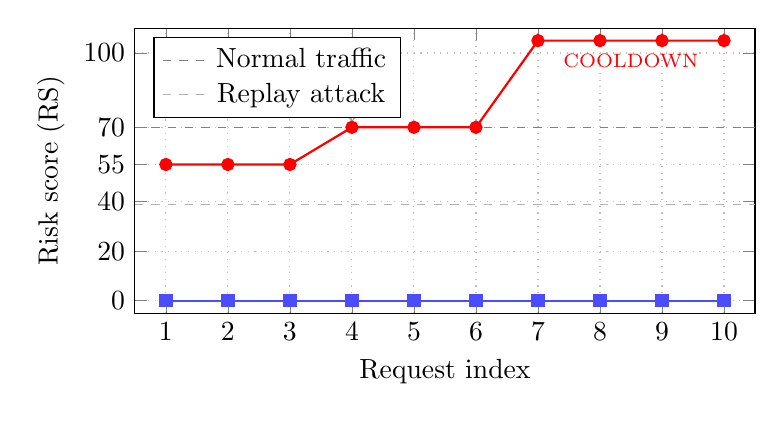
\begin{tikzpicture}
\begin{axis}[
  width=0.78\linewidth, height=5.2cm,
  xlabel={Request index}, ylabel={Risk score (RS)},
  xmin=0.5, xmax=10.5, ymin=-5, ymax=110,
  xtick={1,2,3,4,5,6,7,8,9,10},
  ytick={0,20,40,55,70,100},
  yticklabels={0,20,40,55,70,100},
  legend pos=north west,
  grid=major, grid style={dotted,gray!50},
  every axis plot/.append style={thick},
]
% DENIED threshold line
\addplot[dashed, gray, thin] coordinates {(0.5,70)(10.5,70)};
\node[right, gray, font=\scriptsize] at (axis cs:10.5,70) {DENIED ($>$69)};
% ESCALATED threshold line
\addplot[dashed, gray!60, thin] coordinates {(0.5,39)(10.5,39)};
\node[right, gray!60, font=\scriptsize] at (axis cs:10.5,39) {APPROVED ($\leq$39)};
% Normal traffic (RS=0 throughout)
\addplot[mark=square*, blue!70, solid]
  coordinates { (1,0) (2,0) (3,0) (4,0) (5,0) (6,0) (7,0) (8,0) (9,0) (10,0) };
\addlegendentry{Normal traffic}
% Sequential replay (105 = COOLDOWN sentinel)
\addplot[mark=*, red, solid]
  coordinates { (1,55) (2,55) (3,55) (4,70) (5,70) (6,70) (7,105) (8,105) (9,105) (10,105) };
\addlegendentry{Replay attack}
% COOLDOWN label
\node[red, font=\scriptsize] at (axis cs:8.5,97) {COOLDOWN};
% Rule 3 annotation
\draw[->, gray!70, thin] (axis cs:4,75) -- (axis cs:4,72);
\node[above, gray!70, font=\scriptsize] at (axis cs:4,76) {Rule~3};
\end{axis}
\end{tikzpicture}
\caption{Replay vs.\ normal traffic: RS per request (Case~2 sequential replay).
Requests 1--3: RS~$=55$ (\texttt{ESCALATED}).
Request~4: F\_anom Rule~3 fires (+15 RS) $\to$ RS~$=70$ (\texttt{DENIED}).
Request~7+: \texttt{COOLDOWN\_ACTIVE} (sentinel 105).
Normal traffic stays at RS~$=0$ throughout.}
\label{fig:replay}
\end{figure}

These experiments address the adversarial-robustness and scaling gaps identified
in Section~\ref{sec:evaluation}.
All scripts, raw output, and Redis configuration are available in
\texttt{compliance/adversarial/}.

\subsubsection*{Security Properties Under Adversarial Stress}

We map the evaluated attack strategies to the security properties defined in
Section~\ref{sec:security-model}, analyzing whether each property holds under
adversarial conditions.

\paragraph{Determinism.}
Decision outcomes remain consistent under identical inputs and state conditions,
including under concurrent execution and adversarial request patterns.

\paragraph{Cooldown Enforcement.}
Attack~1 (cooldown evasion via pattern alternation) directly targets the cooldown
mechanism. Results show that cooldown activation cannot be indefinitely avoided:
adversarial alternation delays but does not prevent enforcement. This confirms
that cooldown is eventually enforced under repeated violations.

\paragraph{Bounded Adaptation Resistance.}
Attack~1 also exercises adaptive behavior. The experiment shows that the denial
counter evolves monotonically under repeated violations: \texttt{APPROVED} requests
do not reset prior denials. As a result, adversarial interleaving strategies cannot
asymptotically evade enforcement, establishing a bounded adaptation property.

\paragraph{Per-Agent Isolation.}
Attack~2 (distributed multi-agent attack) targets system-wide coordination. Results
show that ACP enforces constraints independently per agent, maintaining isolation.
However, coordinated behavior across agents is not detected, which constitutes an
explicit design limitation rather than a violation.

\paragraph{State Sensitivity Under Load.}
Attack~3 (state backend contention) evaluates system behavior under adversarial load.
While throughput degrades due to shared state contention, decision correctness and
enforcement properties remain unaffected.

\paragraph{Bounded Replay Resistance.}
Attack~4 (token replay) targets the cryptographic layer, specifically the absence
of nonce tracking in ACP's stateless admission model.
Results confirm that identical replays are detected via F\_anom Rule~3 pattern
accumulation, which escalates borderline-ESCALATED tokens to DENIED after $Y=3$
occurrences in 5~minutes.
Near-identical tokens with varied resource fields evade Rule~3, establishing an
explicit boundary: ACP converts identical replays into observable state transitions
but does not provide strong cryptographic replay prevention.
This is empirically validated; see Section~\ref{sec:limitations} for the
corresponding Limitations note.
The property is summarized: \emph{replay resistance is enforced through temporal
validity and anomaly accumulation, not nonce-based prevention.}

\medskip
\noindent\textbf{Summary.}
The evaluated attacks confirm that ACP enforces its core security properties under
adversarial conditions. No violations are observed; instead, limitations arise from
explicit design trade-offs, particularly in cross-agent correlation.
These results reinforce the central design insight:
\textbf{ACP is compute-cheap but state-sensitive}.

% ── Limitations ───────────────────────────────────────────────────────────────
\subsection{Limitations}
\label{sec:limitations}

The evaluation uses an in-memory state backend for latency benchmarks and a
single-node Docker Redis instance for backend comparison.
Persistent storage, distributed deployments with replication, and wide-area
network latency introduce considerations not measured here.

\textbf{Replay resistance is bounded.}
ACP does not implement nonce-based replay prevention; replay resistance is
enforced through temporal validity (\texttt{TimestampDrift} flag) and anomaly
accumulation (F\_anom Rule~3).
Tokens with varied resource fields and moderate base RS~$<$~DENIED threshold
can evade pattern-based detection while generating \texttt{ESCALATED} outcomes,
preventing cooldown activation (Experiment~4, Case~4).
Nonce tracking requires cryptographic session state that is outside the scope of
ACP's stateless per-request admission model.
This is an explicit design boundary, empirically characterized in Experiment~4.

\subsection{Summary}

These results consistently demonstrate that \textbf{ACP is compute-cheap but state-sensitive.}
Decision evaluation incurs minimal overhead ($\sim$820\,ns), while system throughput is bounded
by the characteristics of the underlying state backend.
The cooldown short-circuit path (88\,ns, 9.5$\times$ faster than full evaluation) demonstrates
that the execution contract's step ordering is a performance-relevant design decision, not only
a correctness one.
These findings highlight the importance of the \texttt{LedgerQuerier} abstraction: protocol
semantics remain stable while deployment performance scales with the quality of the state backend.

\subsection{Roadmap}

\begin{table}[h!]
\centering
\small
\begin{tabular}{@{}ll@{}}
\toprule
\textbf{Item} & \textbf{Status} \\
\midrule
Core specs (L1--L4), 38 documents & Complete \\
Go reference implementation (23 packages) & Complete \\
Conformance test vectors (73 signed + 65 unsigned RISK-2.0) & Complete \\
OpenAPI 3.1.0 (\texttt{openapi/acp-api-1.0.yaml}, 18 endpoints) & Complete \\
Python SDK (\texttt{impl/python/}) & Complete (L1 + full API client) \\
Docker image (\texttt{ghcr.io/chelof100/acp-server:latest}) & Complete \\
Multi-org interoperability demo (\texttt{examples/multi-org-demo/}) & Complete (GAP-14) \\
ACP-RISK-2.0 (F\_anom + Cooldown, \texttt{pkg/risk}) & v1.16 Complete \\
Payment-agent demo (\texttt{examples/payment-agent/}) & v1.16 Complete \\
ACP-SIGN-2.0 spec (Ed25519 + ML-DSA-65 hybrid) & v1.16 Complete \\
ACR-1.0 sequence compliance runner + 5 stateful vectors & v1.17 Complete \\
TLA+ formal model (TLC-runnable, 3 invariants) & v1.17 Complete \\
ACP-SIGN-2.0 HYBRID stub (\texttt{pkg/sign2/}) & v1.17 Complete \\
Performance benchmarks (latency, throughput, state contention) & v1.18 Complete \\
Adversarial evaluation (cooldown evasion, distributed multi-agent, state backend stress) & v1.19 Complete \\
Token replay adversarial evaluation (Experiment~4, F\_anom Rule~3 escalation) & v1.20 Complete \\
Deployment Considerations section (state backend selection, cross-agent boundary, policy tuning) & v1.20 Complete \\
Post-quantum Go implementation (Dilithium, circl) & v1.20 \\
L5 Decentralized (ACP-D) & Specification in design (v2.0) \\
IETF RFC submission & After L5 stabilization \\
\bottomrule
\end{tabular}
\caption{ACP v1.20 development roadmap.}
\end{table}

% ============================================================
\section{Compliance Testing (ACR-1.0 Sequence Runner)}
\label{sec:compliance-testing}
% ============================================================

We introduce a compliance runner, \textbf{ACR-1.0} (ACP Compliance Runner 1.0), that validates ACP-RISK-2.0 implementations
against sequence-based test cases.
The runner operates in two modes: \emph{library mode} (direct call to \texttt{pkg/risk},
no network, deterministic) and \emph{HTTP mode} (external server validation for interoperability).
All 73 signed single-shot conformance vectors plus 5 sequence scenarios
are validated on every commit.

\subsection{Sequence-Based Test Vectors}

Unlike single-shot conformance vectors, sequence-based vectors capture \emph{temporal dynamics}
and emergent risk patterns across multiple requests to the same engine instance.
The compliance runner executes steps in order, maintains state between them
(request history, pattern counts, denial counts, cooldown),
and validates each step's \texttt{decision} and \texttt{risk\_score} against expected values.

The five sequence vectors in \texttt{compliance/test-vectors/sequence/} cover:

\begin{table}[h!]
\centering
\small
\begin{tabular}{@{}llll@{}}
\toprule
\textbf{Vector ID} & \textbf{Steps} & \textbf{Behavior Tested} & \textbf{Key Invariant} \\
\midrule
\texttt{SEQ-BENIGN-001}         & 3 & Benign repeated reads          & Baseline: RS=0, no state buildup \\
\texttt{SEQ-BOUNDARY-001}       & 3 & RS boundary conditions          & Exact thresholds: 0, 25, 35, 40, 70 \\
\texttt{SEQ-PRIVJUMP-001}       & 2 & Low-risk → high-risk jump       & No residual benefit from prior APPROVED \\
\texttt{SEQ-FANOM-RULE3-001}    & 4 & F\_anom Rule~3 activation       & Pattern count $\geq 3$ at step~4 adds $+15$ \\
\texttt{SEQ-COOLDOWN-001}       & 4 & Cooldown trigger and block      & 3 DENIED in 10\,min → cooldown active \\
\bottomrule
\end{tabular}
\caption{ACR-1.0 sequence test vectors. All 5/5 pass in library mode with the Go reference implementation.}
\end{table}

\noindent\textbf{Execution contract.}
The runner implements the execution contract defined by ACP-RISK-2.0:
evaluate first (stateless), then update state.
Critically, \texttt{AddPattern()} is called \emph{after} \texttt{Evaluate()},
so the pattern count visible to step $n$'s evaluation is $n-1$.
F\_anom Rule~3 (pattern count $\geq 3$) therefore first triggers on step~4, not step~3.
This contract is what makes the system testable and verifiable by third parties.

\begin{lstlisting}[language=Go, caption={ACR-1.0 execution contract in library mode.}]
now := time.Now()                                  // capture once
result, _ := risk.Evaluate(req, querier)           // 1: stateless eval
querier.AddRequest(req.AgentID, now)               // 2: always
querier.AddPattern(patKey, now)                    // 3: always (feeds F_anom Rule 3)
if result.Decision == risk.DENIED {
    querier.AddDenial(req.AgentID, now)            // 4: conditional
    if should, _ := risk.ShouldEnterCooldown(...)  // 5: check threshold
        querier.SetCooldown(agentID, now.Add(p))   // 6: set expiry
    }
}
\end{lstlisting}

\subsection{Model--Implementation Alignment}

The TLA+ model, test vectors, and runtime evaluation are aligned through a shared
request abstraction:

\begin{table}[h!]
\centering
\small
\begin{tabular}{@{}lll@{}}
\toprule
\textbf{TLA+ variable} & \textbf{Runner field} & \textbf{Engine field} \\
\midrule
\texttt{capability}, \texttt{resource} & \texttt{RunnerRequest} & \texttt{EvalRequest} \\
\texttt{risk\_score}                   & \texttt{risk\_score}   & \texttt{RSFinal} \\
\texttt{decision}                      & \texttt{decision}      & \texttt{Decision} \\
\texttt{ledger}                        & (audit log)            & \texttt{InMemoryQuerier} events \\
\texttt{cooldown}                      & \texttt{denied\_reason} & \texttt{CooldownActive()} \\
\bottomrule
\end{tabular}
\caption{Alignment across TLA+ formal model, ACR-1.0 runner, and ACP-RISK-2.0 engine.}
\end{table}

% ============================================================
\section{End-to-End Verifiability}
\label{sec:e2e-verifiability}
% ============================================================

ACP~v1.20 enables end-to-end verifiability by aligning formal specification,
test vectors, and runtime validation through a shared request abstraction.
Invariants proven in TLA+ are instantiated as concrete test vectors
and validated empirically by the compliance runner.

\begin{figure}[h!]
\centering
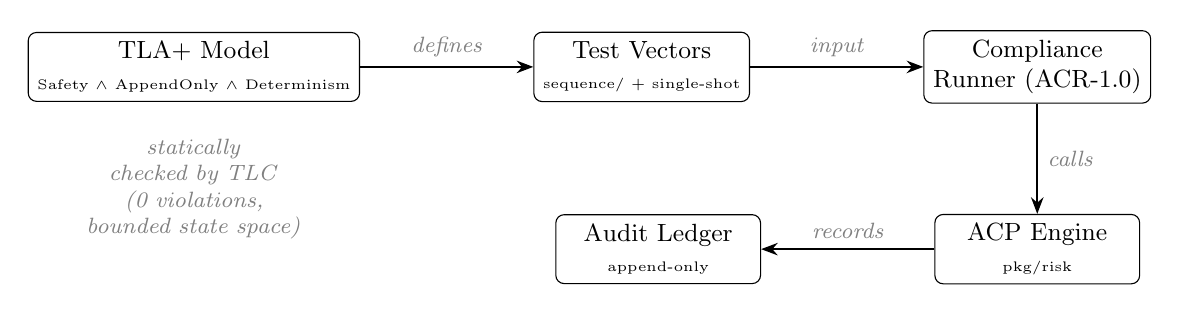
\begin{tikzpicture}[
  node distance=1.4cm and 2.2cm,
  box/.style={draw, rounded corners=3pt, minimum width=2.6cm, minimum height=0.8cm,
              align=center, font=\small},
  arr/.style={-{Stealth[length=6pt]}, thick},
  note/.style={font=\footnotesize\itshape, text=gray}
]
  \node[box] (tla)     {TLA+ Model\\{\tiny Safety $\wedge$ AppendOnly $\wedge$ Determinism}};
  \node[box, right=of tla]    (vec)     {Test Vectors\\{\tiny sequence/ + single-shot}};
  \node[box, right=of vec]    (runner)  {Compliance\\Runner (ACR-1.0)};
  \node[box, below=of runner] (engine)  {ACP Engine\\{\tiny pkg/risk}};
  \node[box, left=of engine]  (ledger)  {Audit Ledger\\{\tiny append-only}};

  \draw[arr] (tla)    -- node[above, note] {defines}  (vec);
  \draw[arr] (vec)    -- node[above, note] {input}     (runner);
  \draw[arr] (runner) -- node[right, note] {calls}     (engine);
  \draw[arr] (engine) -- node[above, note] {records}   (ledger);

  \node[note, below=0.35cm of tla, text width=3cm, align=center]
        {statically checked by TLC\\(0 violations, bounded state space)};
\end{tikzpicture}
\caption{ACP end-to-end verifiability pipeline.
  The TLA+ model defines the invariants that test vectors instantiate and the compliance runner validates at runtime.
  The ACP engine records every decision in the append-only audit ledger.
  The TLA+ layer is a static verification artifact; it does not run at admission time.}
\label{fig:acp-verifiability}
\end{figure}

\noindent What is formally verified in TLA+ holds at runtime.
Each TLA+ invariant is instantiated as a concrete test vector
and validated empirically by the compliance runner.
This is the connection across the three layers of the v1.20 verifiability stack:
formal $\to$ data $\to$ runtime.

% ============================================================
\section{How to Implement ACP}
% ============================================================

ACP is a specification---it does not require adopting any specific platform.
It can be implemented on top of existing infrastructure.

\subsection{Minimum Requirements for L1 Conformance}

\begin{itemize}[noitemsep]
  \item \textbf{Ed25519 public key infrastructure.} Key pair for each agent.
  \item \textbf{JCS implementation (RFC~8785).} Deterministic canonicalization for all signed artifacts.
  \item \textbf{Capability Token issuance and verification} with all mandatory fields per ACP-CT-1.0~\S5.
  \item \textbf{Handshake endpoint} to issue and verify challenges (ACP-HP-1.0~\S6).
  \item \textbf{Capability registry} with the core domains of ACP-CAP-REG-1.0.
\end{itemize}

\subsection{Additional Requirements for L3 Conformance}

\begin{itemize}[noitemsep]
  \item Root Institutional Key held in HSM with documented rotation process.
  \item Registration with an ITA authority (centralized or federated model).
  \item Deterministic risk engine implementing ACP-RISK-2.0 (F\_res, F\_ctx, F\_hist, F\_anom, Cooldown).
  \item Revocation endpoint (Mechanism~A: online endpoint, or Mechanism~B: CRL).
  \item Append-only storage for the Audit Ledger with per-event signing.
  \item Complete HTTP API per ACP-API-1.0, including health and conformance endpoints.
  \item Public conformance declaration at \texttt{GET /acp/v1/conformance}.
\end{itemize}

\subsection{What ACP Does Not Prescribe}

ACP defines the \emph{what}---mechanisms, flows, data structures, requirements.
It does not prescribe the \emph{how} of internal implementation:
programming language, database, HSM provider, ITA provider,
or specific integration with existing RBAC or Zero Trust systems.

% ============================================================
\section{Deployment Considerations}
\label{sec:deployment}
% ============================================================

ACP does not replace higher-level coordination or monitoring systems;
it provides a verifiable admission control primitive within a larger operational stack.
This section characterizes the deployment decisions that adopters must make
when integrating ACP into production infrastructure.

\subsection{State Backend Selection}

The \texttt{LedgerQuerier} interface is the primary deployment decision surface.
The reference \texttt{InMemoryQuerier} is suitable for development, single-process
testing, and conformance evaluation.
Production deployments require an external backend with durability and horizontal
scalability guarantees.

\begin{table}[h!]
\centering\small
\begin{tabular}{llll}
\toprule
Backend & Throughput & Durability & Recommended use \\
\midrule
InMemoryQuerier   & $\sim$920k req/s  & None (process-local) & Dev / conformance testing \\
Redis sorted sets & $\sim$2{,}100 req/s (unpipelined) & AOF/RDB & Multi-process, low-latency \\
Redis + pipelining / Lua & $\gg$2{,}100 req/s & AOF/RDB & High-throughput production \\
Postgres / MySQL  & Backend-dependent & Full ACID & Audit-grade persistence \\
\bottomrule
\end{tabular}
\caption{LedgerQuerier backend options.
The admission control logic (\texttt{pkg/risk.Evaluate}) is stateless and backend-agnostic;
all state transitions are delegated to the LedgerQuerier abstraction.
Redis throughput measured in Experiment~3 (single-command, no pipelining, Docker loopback).}
\label{tab:backends}
\end{table}

The key architectural property is that the ACP decision function is compute-cheap
and the throughput ceiling is set entirely by the state backend.
Replacing the backend does not require modifying the admission control logic
or redeploying the protocol layer.

\subsection{Agent Identity Provisioning}

ACP requires a stable \texttt{agent\_id} per agent instance.
Provisioning can be integrated with existing IAM or service mesh identity systems:
the \texttt{agent\_id} is an opaque string from ACP's perspective,
provided it is unique, stable across requests, and included in signed capability tokens.
Key pairs (Ed25519 for L1--L4) should be provisioned at agent registration time
and rotated according to the organization's key management policy.

\subsection{Multi-Organization Boundaries}

Each organization deploys its own ACP instance with a sovereign Institutional Key.
Admission control decisions are evaluated locally against the deploying organization's
\texttt{LedgerQuerier} and \texttt{PolicyConfig}.
Cross-organization request flows are handled by ACP-CROSS-ORG-1.0:
the receiving organization evaluates the incoming execution token independently,
applying its own risk policy and local ledger state.

Federated deployments use mutual recognition (ACP-ITA-1.1) to establish
cross-org trust anchors without requiring a shared root of trust.
The per-org isolation model is intentional: an organization's admission control
decisions are not visible to or affected by another organization's ledger.

\subsection{Cross-Agent Coordination (L3)}

ACP enforces admission control \emph{per agent} and \emph{per request}.
When multiple agents collaborate on a composite task,
each agent's admission request is evaluated independently against its own
\texttt{agent\_id}, capability token, and ledger history.

ACP does not implement cross-agent correlation or orchestration-level coordination.
This is an explicit scope boundary: as demonstrated in Experiment~2 (§\ref{sec:adversarial}),
a coordinated group of $N$ agents can collectively execute $3N$ high-risk requests before
all agents are individually blocked.
Mitigating coordinated multi-agent threats requires attribution at the orchestration layer
(e.g., shared-resource rate limits, agent group policies, identity clustering),
which ACP is designed to \emph{complement}, not replace.

The ACP-CROSS-ORG-1.0 interaction model provides a protocol-level primitive for
multi-organization agent coordination; full L3 cross-agent orchestration is
a deployment-layer concern outside the scope of this specification.

\subsection{Integration with Existing Infrastructure}

ACP occupies the Execution Governance layer of the Agent Governance Stack
(Section~\ref{sec:design-insight}).
It is designed to complement---not replace---existing access control and
observability infrastructure:

\begin{itemize}[noitemsep]
  \item \textbf{RBAC / ABAC / OPA:} ACP provides per-request admission control with
    temporal state (history, cooldown). Existing resource-authorization systems
    continue to apply \emph{after} ACP admission succeeds.
  \item \textbf{Zero Trust:} Environmental signals (\texttt{external\_ip},
    \texttt{off\_hours}, \texttt{geo\_outside}, \texttt{untrusted\_device})
    integrate Zero Trust context directly into the ACP risk score via F\_ctx.
  \item \textbf{SIEM / Observability:} The Audit Ledger (ACP-LEDGER-1.3) produces
    per-decision signed records suitable for ingestion into log aggregation pipelines.
    Each entry carries a \texttt{policy\_hash} enabling post-hoc attribution of
    decisions to specific policy versions.
  \item \textbf{Monitoring systems:} ACP's cooldown and escalation events are
    observable state transitions---not silent blocks. They are designed to be
    surfaced to monitoring systems for incident response.
\end{itemize}

\subsection{Policy Tuning}

The \texttt{PolicyConfig} parameters (defaults documented in ACP-RISK-2.0 Appendix~A
and exposed via \texttt{DefaultPolicyConfig()}) are the primary operational levers:

\begin{itemize}[noitemsep]
  \item \texttt{CooldownPeriodSeconds}: Tune based on threat model.
    Shorter ($<300$s) enables faster recovery for false positives;
    longer ($\geq600$s) provides stronger containment under sustained attack.
  \item \texttt{CooldownTriggerDenials}: Lower values ($=2$) increase sensitivity
    at the cost of higher false-positive rate; higher values allow more free denials
    before containment.
  \item \texttt{AnomalyRule3ThresholdY}: Controls the pattern-accumulation window.
    Default $Y=3$ balances replay detection latency against false positives from
    legitimate repeated requests (e.g., polling agents).
  \item \texttt{PolicyHash}: Pin policy versions in capability tokens to prevent
    silent policy changes from altering admission decisions post-issuance.
\end{itemize}

\noindent ACP provides sensible defaults via \texttt{DefaultPolicyConfig()}
(Appendix~A of ACP-RISK-2.0).
Organizations should treat policy calibration as an operational process,
informed by observed denial rates, throughput baselines, and threat model requirements.

% ============================================================
\section{Security Model}
\label{sec:security-model}
% ============================================================

This section defines the adversary model and the security properties provided by ACP.

\subsection{Adversary Capabilities}

We consider a probabilistic adversary $\mathcal{A}$ interacting with the system through
agent requests. The adversary is assumed to have the following capabilities:

\begin{itemize}[noitemsep]
  \item \textbf{Request control:} $\mathcal{A}$ can generate arbitrary sequences of requests
    on behalf of one or more agents, including high-frequency and adversarial patterns.
  \item \textbf{Adaptive behavior:} $\mathcal{A}$ can adapt future requests based on past
    responses (approval/denial outcomes), enabling iterative probing strategies.
  \item \textbf{Multi-agent coordination:} $\mathcal{A}$ may coordinate multiple agents to
    attempt distributed evasion, including alternating identities or cross-agent patterns.
  \item \textbf{Input manipulation:} $\mathcal{A}$ can choose all request fields
    (capability, resource, context) within the bounds of the protocol specification.
\end{itemize}

\subsection{Adversary Limitations}

The following components are trusted and cannot be modified by the adversary:

\begin{itemize}[noitemsep]
  \item \textbf{Execution contract:} the sequence of operations governing state updates
    (evaluation followed by state transitions) is enforced correctly.
  \item \textbf{State integrity:} the underlying state backend (ledger, cooldown state,
    pattern counters) is append-only and tamper-resistant.
  \item \textbf{Evaluation function:} the decision function (ACP-RISK-2.0) is deterministic
    and correctly implemented.
  \item \textbf{Cryptographic primitives:} signature verification and identity binding are
    assumed secure under standard assumptions (EUF-CMA security of Ed25519).
\end{itemize}

This model corresponds to an adversary that can fully control inputs but cannot compromise
the integrity of the control system itself.

\subsection{Security Properties}

Under this model, ACP enforces the following properties:

\paragraph{Determinism.}
For a given request and system state, the evaluation function produces a unique and
reproducible decision outcome.
This prevents adversarial exploitation of non-determinism.
The \texttt{RiskDeterminism} invariant in the TLA+ model formally specifies this property.

\paragraph{State Consistency.}
All state transitions follow the execution contract, ensuring that historical behavior
is consistently reflected in future decisions.

\paragraph{Cooldown Enforcement.}
An adversary cannot bypass cooldown mechanisms through repeated or adaptive requests.
Once cooldown conditions are met, subsequent requests are deterministically denied within
the cooldown window, regardless of request content.
This is confirmed by the \texttt{SEQ-COOLDOWN-001} sequence test vector.

\paragraph{History Integrity.}
Past decisions and events cannot be modified or removed.
The append-only ledger (ACP-LEDGER-1.3) and the \texttt{LedgerAppendOnlyTemporal} TLA+ invariant
formally guarantee monotonic accumulation of historical state.

\paragraph{Bounded Adaptation Resistance.}
While $\mathcal{A}$ may adapt request patterns, such adaptations cannot eliminate the influence
of accumulated history (repeated denials, pattern counts) on future decisions.
In particular, the denial counter evolves monotonically: intervening approved requests
do not reset prior denials, ensuring eventual enforcement under repeated violations.

\paragraph{Per-Agent Isolation.}
Policy enforcement is applied independently per agent.
Actions by one agent do not affect the enforcement state of another.
This property bounds the impact of a compromised or malicious agent to its own
request history.

\subsection{Informal Security Argument}

Because ACP separates stateless evaluation from state management and enforces a strict
execution contract, every request results in a deterministic state transition that cannot
be bypassed.
The append-only nature of the state backend ensures that historical information accumulates
monotonically: cooldown activation follows deterministic threshold conditions applied to
accumulated state; repeated probing eventually triggers enforced denial periods.

Because decisions are reproducible given the same input sequence and initial state,
any observed behavior can be externally verified.
This limits $\mathcal{A}$'s ability to exploit hidden or undocumented system behavior.

\subsection{Limitations}

The security guarantees of ACP rely on the integrity of the execution environment:

\begin{itemize}[noitemsep]
  \item Compromise of the state backend (deletion or modification of history) breaks core guarantees.
  \item Incorrect implementation of the execution contract may lead to inconsistent behavior.
  \item The model does not address side-channel attacks or network-level adversaries.
  \item Post-quantum signature migration (ACP-SIGN-2.0 HYBRID, Ed25519 $\to$ ML-DSA-65)
    is specified and stubbed; full implementation is deferred to v1.20.
\end{itemize}

ACP is therefore best understood as a control-layer mechanism that assumes a trusted
execution and storage environment, while providing strong guarantees on decision consistency
and temporal behavior under adversarial inputs.

% ============================================================
\section{Related Work}
\label{sec:related-work}
% ============================================================

\subsection{Access Control and Policy Enforcement}

Traditional access control models such as Role-Based Access Control (RBAC)~\cite{sandhu1996rbac}
and Attribute-Based Access Control (ABAC)~\cite{hu2015abac} provide structured mechanisms for
regulating access decisions based on predefined roles or attributes.
Policy languages such as XACML~\cite{oasis2013xacml} and modern policy engines such as
Open Policy Agent~\cite{opa} and Cedar~\cite{cedar} extend these paradigms with expressive
evaluation engines.

These systems are fundamentally designed around \emph{stateless decision evaluation}:
they evaluate a request against policy at a single point in time.
They do not define how system state evolves as a result of decisions over time,
and they do not formalize how historical behavior (repeated denials, temporal patterns)
influences subsequent decisions in a deterministic and auditable manner.

ACP differs by explicitly separating:
(i)~stateless decision evaluation,
(ii)~externalized state management, and
(iii)~an execution contract governing state evolution across requests.
This enables reasoning not only about individual decisions, but about the temporal behavior
of the admission system.

\subsection{Runtime Policy Systems and Agent Frameworks}

Recent protocols for autonomous agents and multi-agent coordination define structured interactions
between components and services.
The Model Context Protocol (MCP)~\cite{mcp} provides structured tool access between LLM applications and services.
Agent-to-Agent (A2A)~\cite{a2a} defines communication and task delegation between agents.

While these protocols address interoperability and orchestration, they do not define:
\begin{itemize}[noitemsep]
  \item a deterministic risk evaluation model that accumulates state across requests,
  \item explicit state evolution semantics with a testable execution contract, or
  \item externally verifiable execution traces that can be reproduced by third parties.
\end{itemize}

Recent work has begun to address security governance for LLM-based agentic systems.
Syros et al.~\cite{syros2025saga} propose SAGA, a security architecture that provides
user-controlled access policies and cryptographic mediation for agent-to-agent tool use
and inter-agent communication.
ACP complements this line of work by focusing on deterministic, auditable admission
control at the individual request level: rather than governing inter-agent communication
channels, ACP enforces stateful risk evaluation and cooldown constraints on each action
request, with an externally verifiable execution contract and formal invariants.
Tsai and Bagdasarian~\cite{tsai2025contextual} argue at HotOS~2025 that security policies
must be purpose-specific rather than uniformly applied, emphasising that one-size-fits-all
approaches are inadequate for diverse agent deployments---a perspective consistent with
ACP's per-agent isolation and stateful enforcement boundaries.

ACP complements these approaches by providing a governance layer that is independent of
orchestration protocols, focusing specifically on verifiable decision enforcement and auditability.

\subsection{Auditability and Tamper-Evident Logs}

Secure audit logging~\cite{schneier1999secure} and event sourcing~\cite{fowler2005event} ensure
that past events can be reconstructed and verified after the fact.
These approaches operate \emph{post hoc}: they provide evidence of what occurred without
constraining system behavior in real time.

ACP integrates auditability directly into the admission process.
Every decision---APPROVED, ESCALATED, or DENIED---is recorded in an append-only, cryptographically
chained ledger (ACP-LEDGER-1.3) before the governed action executes.
This enables both real-time enforcement and post-hoc verification from the same artifact.
The \texttt{LedgerAppendOnlyTemporal} invariant in the TLA+ model formally specifies
that ledger entries are never modified or removed.

\subsection{Formal Verification of Protocols}

Model checking~\cite{lamport2002specifying} and symbolic reasoning are used to establish
correctness properties in distributed systems and protocols, typically focusing on safety
and liveness of state transitions.

ACP incorporates formal methods in a targeted manner:
the TLA+ model (\texttt{tla/ACP.tla}) mechanically checks three critical invariants
(fail-closed admission, append-only ledger, risk determinism) using TLC.
Rather than attempting full-system verification, ACP adopts a pragmatic approach in which
formally verified invariants are instantiated as concrete sequence test vectors
and validated at runtime by the ACR-1.0 compliance runner.
This creates a three-layer verifiability chain: formal $\to$ data $\to$ runtime.

\subsection{Summary}

Table~\ref{tab:comparison} summarizes the properties of ACP relative to existing approaches.

\begin{table}[h!]
\centering
\small
\begin{tabular}{@{}lcccccc@{}}
\toprule
\textbf{Property} & \textbf{RBAC} & \textbf{ABAC} & \textbf{OPA} & \textbf{Cedar} & \textbf{MCP/A2A} & \textbf{ACP} \\
\midrule
Stateful decisions       & \no & \no & \no & \no & \no & \yes \\
Deterministic evaluation & \yes & \yes & \yes & \yes & \no & \yes \\
Auditability             & partial & partial & partial & partial & \no & \yes \\
Runtime enforcement      & \yes & \yes & \yes & \yes & partial & \yes \\
Temporal behavior        & \no & \no & \no & \no & \no & \yes \\
External verifiability   & \no & \no & \no & \no & \no & \yes \\
Execution contract       & \no & \no & \no & \no & \no & \yes \\
Agent-native             & \no & \no & \no & \no & partial & \yes \\
\bottomrule
\end{tabular}
\caption{Comparison of ACP with existing access control and agent governance approaches.
\yes~=~fully supported; \no~=~not supported; partial~=~partially addressed.}
\label{tab:comparison}
\end{table}

Existing systems address individual aspects of the problem---policy evaluation,
agent orchestration, audit logging, or formal verification.
ACP's contribution lies in combining these elements into a unified model centered on
an explicit execution contract.
This enables a property not directly provided by prior systems:
the ability to deterministically reproduce and externally verify the behavior of
an admission decision system over time.

Unlike existing systems, ACP explicitly models temporal behavior---history accumulation,
anomaly detection, and cooldown enforcement---within the admission decision itself,
and provides verifiable execution semantics through signed test vectors and a runtime compliance runner.
This combination of temporal state, runtime enforcement, and external verifiability
is not jointly addressed by any prior system in Table~\ref{tab:comparison}.

% ============================================================
\section{Conclusion}
% ============================================================

Autonomous agents are already operating in institutional environments.
The question is not whether they will operate---it is whether they will do so with or without formal governance.
ACP proposes that they operate with formal governance, with verifiable mechanisms,
and with traceability that can withstand an external audit.

ACP is not the first attempt to control autonomous agents.
It is the first attempt to do so through a formal technical specification with precise state models,
demonstrable security properties, and verifiable conformance requirements.
The difference between a best-practices policy and a formal protocol is exactly that:
behaviors are defined, failures have specific error codes, and conformance can be verified.

The goal of ACP is not to make agents more capable. It is to make them governable.
That is a necessary condition for their institutional deployment to be sustainable at scale.

ACP does not eliminate all sources of failure in distributed agent systems.
It does not prescribe network transport, consensus mechanisms, or business-level dispute resolution.
What it provides is a structured, auditable, and formally specified model for
admission control, delegation, revocation, and cross-organization interaction---
the layer that existing identity and policy frameworks leave unaddressed.

The v1.20 specification is complete.
A full Go reference implementation (23 packages, L1--L4), 73 signed + 65 unsigned RISK-2.0 conformance test vectors,
5 stateful sequence test vectors (ACR-1.0 compliance runner),
a TLC-runnable TLA+ formal model (3 invariants, 0 violations),
an ACP-SIGN-2.0 HYBRID mode stub with Ed25519 and ML-DSA-65 migration path,
an executable multi-organization interoperability demo (\texttt{examples/multi-org-demo/}),
a payment-agent killer demo (\texttt{examples/payment-agent/}),
an extended OpenAPI 3.1.0 specification (18 endpoints),
and adversarial evaluation across four attack scenarios including token replay (Experiment~4)
are publicly available at \url{https://github.com/chelof100/acp-framework-en}.\\
\textbf{Preprint:} \url{https://arxiv.org/abs/2603.18829} \quad \textbf{Zenodo:} \href{https://doi.org/10.5281/zenodo.19219776}{10.5281/zenodo.19219776}\\
The specification and implementation are open for technical review, pilot implementation, and formal standardization.

TraslaIA invites organizations interested in adopting ACP, contributing to its evolution,
or participating in the standardization process to reach out directly.

ACP demonstrates that admission control for autonomous agents can be both computationally
efficient and operationally enforceable---provided that decision logic and state management
are cleanly separated. The protocol is \textbf{compute-cheap but state-sensitive}: the
\texttt{LedgerQuerier} abstraction keeps the evaluation function at $\sim$820\,ns while
allowing the state backend to be replaced, optimized, or scaled independently.
This is not an implementation detail---it is the architectural property that makes ACP
deployable in production without sacrificing governance correctness.

\bigskip
\noindent\textbf{Marcelo Fernandez | TraslaIA}\\
\texttt{info@traslaia.com} | \url{https://agentcontrolprotocol.xyz}

% ============================================================
\appendix
\section{Glossary}
% ============================================================

\begin{table}[h!]
\centering
\small
\begin{tabular}{@{}lp{10cm}@{}}
\toprule
\textbf{Term} & \textbf{Definition} \\
\midrule
ACR-1.0 & ACP Compliance Runner 1.0. Sequence-based test runner for ACP-RISK-2.0. Distinct from ACP-CR-1.0 (Change Request Process governance document). \\
AgentID & Cryptographic identifier: \texttt{base58(SHA-256(Ed25519\_public\_key))}. Immutable and unforgeable. \\
Capability Token (CT) & Signed JSON artifact authorizing an agent to perform specific actions on a defined resource during a limited period. \\
Execution Token (ET) & Single-use artifact issued after an APPROVED decision. Authorizes exactly that action at that moment. \\
ITA & Institutional Trust Anchor. Authoritative registry linking \texttt{institution\_id} to institutional Ed25519 public key. \\
RIK & Root Institutional Key. Institution's Ed25519 key pair held in HSM. \\
Risk Score (RS) & Integer in $[0, 100]$ produced by the deterministic risk function. Determines the authorization decision. \\
Autonomy Level & Integer 0--4 assigned to an agent determining applicable risk evaluation thresholds. \\
PoP & Proof-of-Possession. Cryptographic proof that the bearer of a CT possesses the corresponding private key. \\
Audit Ledger & Chain of signed events where $h_n = \text{SHA-256}(e_n \| h_{n-1})$. Append-only and immutable. \\
MRA & Mutual Recognition Agreement. Bilateral document signed by two ITA authorities for cross-authority interoperability. \\
ESCALATED & ACP decision when RS is in the intermediate range. Action not executed until explicit resolution. \\
Fail Closed & Design principle: on any internal failure, the action is denied. Never approved by default. \\
\bottomrule
\end{tabular}
\caption{ACP Glossary.}
\end{table}

% ============================================================
\section{Formal Verification (ACP-RISK-2.0 — TLC-Runnable)}
\label{app:tlaplus}
% ============================================================

The \texttt{tla/ACP.tla} module is a complete TLC-runnable TLA+ model of the ACP-RISK-2.0
admission control engine.
It checks three invariants over a bounded state space
(2 agents $\times$ 4 capabilities $\times$ 3 resources, ledger depth $\leq 5$):

\begin{verbatim}
---- MODULE ACP ----
EXTENDS Sequences, Integers, TLC

CONSTANTS Agents, Capabilities, Resources

CapabilityBase(cap) ==
    CASE cap = "admin"     -> 60
      [] cap = "financial" -> 35
      [] cap = "write"     -> 10
      [] cap = "read"      -> 0
      [] OTHER             -> 20

ResourceScore(res) ==
    CASE res = "restricted" -> 45
      [] res = "sensitive"  -> 15
      [] res = "public"     -> 0
      [] OTHER              -> 0

ComputeRisk(cap, res) ==
    LET raw == CapabilityBase(cap) + ResourceScore(res)
    IN IF raw > 100 THEN 100 ELSE raw

Decide(rs) ==
    IF      rs >= 70 THEN "DENIED"
    ELSE IF rs >= 40 THEN "ESCALATED"
    ELSE                  "APPROVED"

VARIABLE ledger
INIT == ledger = << >>

EvaluateRequest(a, cap, res) ==
    /\ Len(ledger) < 5
    /\ ledger' = Append(ledger,
            [ agent      |-> a,
              capability |-> cap,
              resource   |-> res,
              risk_score |-> ComputeRisk(cap, res),
              decision   |-> Decide(ComputeRisk(cap, res)) ])

NEXT == \E a \in Agents, cap \in Capabilities, res \in Resources :
            EvaluateRequest(a, cap, res)

Spec == INIT /\ [][NEXT]_ledger

Safety ==
    \A i \in 1..Len(ledger) :
        ledger[i].decision = "APPROVED" => ledger[i].risk_score <= 39

LedgerAppendOnly ==
    \A i \in 1..Len(ledger) :
        /\ ledger[i].decision \in {"APPROVED", "ESCALATED", "DENIED"}
        /\ ledger[i].risk_score >= 0

RiskDeterminism ==
    \A i \in 1..Len(ledger) :
        \A j \in 1..Len(ledger) :
            ( ledger[i].capability = ledger[j].capability
           /\ ledger[i].resource   = ledger[j].resource )
            =>
            ledger[i].risk_score = ledger[j].risk_score

LedgerAppendOnlyTemporal ==
    [][ /\ Len(ledger') >= Len(ledger)
        /\ \A i \in 1..Len(ledger) : ledger'[i] = ledger[i] ]_ledger
====
\end{verbatim}

\noindent\textbf{TLC result.}
Running \texttt{java -jar tla2tools.jar -config ACP.cfg ACP.tla} with
$|\mathit{Agents}|=2$, $|\mathit{Capabilities}|=4$, $|\mathit{Resources}|=3$,
ledger bound~$=5$ produces:
\textit{Model checking completed. No error has been found.}
All four declared invariants/properties (\texttt{TypeInvariant}, \texttt{Safety},
\texttt{LedgerAppendOnly}, \texttt{RiskDeterminism}) and the temporal property
\texttt{LedgerAppendOnlyTemporal} hold over the full reachable state space.

\noindent\textbf{Interpretation.}
\textit{Safety} encodes fail-closed admission: every APPROVED decision had $\mathit{RS} \leq 39$.
\textit{LedgerAppendOnly} encodes tamper-evidence in a state-based view:
every ledger entry carries a valid decision and a non-negative risk score.
\textit{LedgerAppendOnlyTemporal} is the temporal statement: in every step,
existing entries are preserved and the ledger never shrinks.
\textit{RiskDeterminism} is the central invariant of ACP-RISK-2.0: identical
(capability, resource) pairs always produce identical risk scores,
enabling third-party recalculation from a signed policy snapshot.

\noindent\textbf{Scope of the formal model.}
The TLA+ model intentionally focuses on the deterministic core of the protocol---admission
evaluation, ledger append-only property, and risk score determinism---and does not cover all
operational aspects of ACP. Behavioral properties such as cooldown state transitions,
multi-step delegation sequences, and anomaly counter evolution are verified empirically through
the ACR-1.0 sequence compliance runner and its five stateful test vectors.
Extension of the formal model to cover these behaviors is left for future work.

% ============================================================
\section*{Acknowledgements}
% ============================================================

The ACP specification emerged from analysis of operational challenges in deploying autonomous agents in regulated B2B environments.
The protocol design was informed by the IETF RFC process, the Kubernetes admission control architecture,
and the SPIFFE/SPIRE workload identity model.

% ============================================================
% Bibliography
% ============================================================

\bibliographystyle{plain}
\bibliography{references}

\end{document}
